% !TeX root = RJwrapper.tex
\title{ODRF: An R Package for Oblique Decision Tree and Its Random Forest}
\author{by Yu Liu and Yingcun Xia}

\maketitle

\abstract{
	The classification and regression tree (CART) and Random Forest (RF) are popular machine learning methods that involve selecting one predictor at a time as the splitting variable for each node.
	The use of linear combinations of predictors as splitting variables is one of the popular extensions of CART and RF, known as Oblique Decision Trees ({ODT}), and hence ODT-based Random Forests ({ODRF}). Recent studies have also shown the theoretical advantages of {ODT} and {ODRF} over {CART} and {RF}. However, there is still no integrated and efficient software package that can demonstrate the numerical advantages of {ODT} and {ODRF}. To fill this gap, we make several modifications to the existing algorithms and develop an  {R} package \CRANpkg{ODRF} for both \fct{ODT} and \fct{ODRF}. {In addition, the R package includes a series of new functions, such as ODT-based boosting trees (BODT), the ensemble version of BODT (ODBT), ODT visualization (plot.ODT), and an online update function for ODT (online.ODT).} The main part of {ODRF} is executed using the \CRANpkg{Rcpp} package. This paper presents the basic idea of our modifications and illustrates the use of the package. Through numerical experiments, {ODRF} was compared with other packages of decision trees and forests, showing a clear overall improvement in classification and regression tasks.
}

\section{Introduction} \label{sec:intro}

The Classification and Regression Tree (CART) proposed by Professor Leo Breiman \citep{1984Classification} has attracted a great deal of attention from statisticians and data analysts of other disciplines. The method is widely used because it is easy to train and the resulting tree makes the analysis results easy to visualize and interpret \citep{2014Learning}. On the other hand, much attention has been paid to the algorithm and many improvements have been proposed. Classification and regression trees  \citep[{CART}]{quinlan1987decision} and {C4.5} \citep{quinlan1993program} are perhaps the most commonly used decision trees. There is a long list of other decision trees, including the Evolutionary Learning of Globally Optimal Classification and Regression Trees  \citep[{EVT}]{Grubinger2014ectree},  Conditional Inference Trees \citep[CT]{hothorn2006unbiased}, Extremely randomized trees \citep[{ERT}]{2006Extremely}, Model-Based Recursive Partitioning  \citep[{MOB}]{zeileis2015parties}, Bayesian additive regression trees \citep[({BART}) ]{maia2022gp} and generalized linear mixed-model trees  \citep[{glmertree}]{2020Generalized}.  The Random Forests \citep[RF]{breiman2001random}, which is an ensemble of trees by either feature bagging or boosting,  is arguably one of the most efficient machine learning methods, especially for the tabular data \citep{tabularDATA}. Again, there are many ensemble methods that are based on different decision trees, for example, Conditional Random Forests \citep[{cforest}]{hothorn2006unbiased}, Learning Nonlinear Functions Using Regularized Greedy Forest \citep[{RGF}]{2014Learning} and Generalized Random Forest \citep[{GRF}]{athey2019generalized}.

One of the most appealing extensions to CART is the use of linear combinations of the predictors as splitting variables that is known as the Oblique Decision Tree  \citep[{ODT}]{Heath93inductionof}. Recently, \citet{zhan2022consistency} proved the consistency of {ODT} and its random forest ({ODRF}) for very general regression functions as long as they  are continuous, while CART or RF are consistent mainly for regressions with special structures such as additive models.  Again, ensemble can be made based on ODT, resulting in the Oblique-type Random Forests, including Random Rotation Random Forest ({RotRF}) of \cite{blaser2016random}, Random Projection Forests ({RPFs}) of \citet{lee2015fast} and Sparse Projection Oblique Randomer Forests (SPORF) of \cite{tomita2020sparse}. Another type of random forests is the model-based oblique decision forest,  including mainly Canonical Correlation Forests ({CCF}) with classic correlation analysis \citep{rainforth2015canonical},  projection pursuit forest ({PPF}) with linear discriminant analysis \citep{silva2021projection}, oblique random forests ({ORF}) with ridge regression \citep{menze2011oblique}, oblique random survival forests  \citep[{ORSF}]{jaeger2022accelerated} and Heterogeneous oblique random forest \citep[{HORF}]{katuwal2020heterogeneous}. {However, a primary limitation of these oblique methods lies in their computational intensity. To address this issue, \citet{HHCART} introduced a novel algorithm named ``HHCART'', which utilizes Householder matrices to reflect training data at non-terminal nodes. Subsequently, \citet{HHCARTR} developed an accompanying R package \CRANpkg{hhcartr} for both classification and regression tasks.}

In parallel with these developments, Gradient Boosting Trees (GBT) have emerged as another powerful machine learning paradigm. The GBT algorithm was first introduced by \cite{friedman2001greedy}, establishing a powerful framework for supervised learning by sequentially fitting weak learners (typically decision trees) to the residuals of previous models. To address overfitting, \cite{friedman2002stochastic} later proposed stochastic gradient boosting, which incorporates regularization by subsampling both observations and features.
Further enhancements tailored to tree-based models were introduced through modern implementations such as XGBoost \citep{chen2016xgboost}, LightGBM \citep{ke2017lightgbm}, and CatBoost \citep{prokhorenkova2018catboost}. These frameworks optimize tree growth strategies, efficiently handle categorical variables, and significantly improve computational scalability.
Traditionally, boosting algorithms employed axis-aligned splits (as in CART-style trees). However, recent research has explored Oblique Decision Trees (ODT) within boosting frameworks, resulting in Boosting Oblique Decision Trees (BODT). Integrating BODT with randomization techniques, such as random projections \citep{lee2015fast}, further enhances robustness and generalizability.
Notably, our recent work demonstrated that ensembles based on BODT achieve consistency for general continuous regression functions, in contrast to traditional CART-based ensembles that require additive or structured assumptions.

Although the theoretical advantages of oblique decision trees and their random forests have been well understood, the existing packages implementing those extensions only show their better numerical performance in some special cases, and thus have not commonly received and have not got  much  popularity as the methods deserve. {As a consequence, the conventional packages \CRANpkg{rpart} \citep{rpart} of \cite{2000Therneau} for CART and \CRANpkg{randomForest} \citep{RF} of \cite{randomForest} for RF are still the most commonly used packages. The main difficulty in implementing {ODT} or {ODRF} is the estimation of the coefficient, $ \theta $, for the linear combinations, which is also one of the main differences amongst all the existing packages. The estimation methods  of $ \theta $ include random projection, logistic regression, dimension reduction and many others. For example, package \CRANpkg{rerf} \citep{rerf} of \cite{tomita2020sparse} uses random projections; package \CRANpkg{PPforest}  \citep{PPforest} of \cite{silva2021projection} uses linear discriminant and penalized discriminant analysis; 
package \CRANpkg{obliqueRF}  \citep{obliqueRF} of \cite{menze2011oblique}  uses
the partial least squares regression,  logistic regression, and random projection   to find the projections.}
On the other hand, most of the existing {R} packages for such types of random forests can only be used for classification. 
Some of the {R} packages have been removed from the Comprehensive {R} Archive Network (CRAN) at \url{https://CRAN.R-project.org/}. {For comprehensive details, see Table~\ref{Rpackage}, which presents a comparative analysis of nine R packages implementing oblique tree methods. The evaluation assesses their support for six specific functionalities and determines whether they remain available on CRAN.}

Our package, called \CRANpkg{ODRF},  is written based on the above-mentioned packages and the recent work of  \citet{zhan2022consistency}.
In \CRANpkg{ODRF}, the projection pursuit regression \citep{friedman1981projection} is used to find $ \theta $; the details will be stated in the following section. Other options for the estimations of projections are also  provided in the package. 
Compared with the existing random forests, the advantages of \CRANpkg{ODRF} are as follows.
\begin{itemize}

	\item \CRANpkg{ODRF} can be used for both classification and regression, while most existing packages of oblique-type trees or forests can only be used for classification.
	\item Both the tree (\code{ODT}) and random forests (\code{ODRF}) of \CRANpkg{ODRF} have better overall accuracy than existing trees and forests, including traditional CART and RF and other oblique trees or forests.

	\item \CRANpkg{ODRF} allows users to define their own functions to find the projections  at each node, which is essential to the performance of the forests.

	\item \CRANpkg{ODRF} provides an \code{online} class of functions that facilitate the application to streaming data, enabling continuous updates and improvements to existing trees or random forests. 

    \item \CRANpkg{ODRF} develops a new ensemble method (ODBT), 
    which builds random forests of ODT-based boosting trees and outperforms traditional boosting trees and random forests in both classification and regression tasks.

     \item \CRANpkg{ODRF} proposes an innovative approach for constructing linear model trees by incorporating LASSO regularization, while distinctly separating the sets of variables used for node splitting and model fitting.

\end{itemize}

\begin{table}[htbp]
	\centering
	\begin{minipage}{\textwidth}
		\setlength{\tabcolsep}{1.4mm}
		{
			\begin{tabular}{lccccccc}
				\toprule
				& classification & regression & forests & boosting & custom& online & CRAN \\
				&  &  &  &  & splits & updating &  \\
				\midrule
				oblique.tree & \usym{2714}    & \usym{2718}     & \usym{2718}     &\usym{2718}      & \usym{2718}      &\usym{2718}     & \usym{2718}  \\
				pptreeviz & \usym{2713}      & \usym{2718}      & \usym{2718}    & \usym{2718}     & \usym{2718}     & \usym{2718}     & \usym{2714} \\
				PPtreereg & \usym{2718}     & \usym{2714}    & \usym{2718}     & \usym{2718}      &\usym{2718}      & \usym{2718}     & \usym{2718}  \\
				%	hhcartr & \usym{2714}     & N     & N     & N     & N     & N     & N \\
				rotationForest & \usym{2714}     & \usym{2718}     & \usym{2714}     & \usym{2718}      & \usym{2718}     & \usym{2718}      & \usym{2714} \\
				rerf  & \usym{2714}    & \usym{2718}    & \usym{2714}   & \usym{2718}     &\usym{2718}      & \usym{2718}     & \usym{2718}  \\
				PPforest & \usym{2714}     & \usym{2718}     & \usym{2714}     & \usym{2718}     &\usym{2718}     & \usym{2718}  & \usym{2714} \\
				obliqueRF & \usym{2714}    & \usym{2718}     & \usym{2714}     & \usym{2718}     &\usym{2718}     & \usym{2718}      & \usym{2718}  \\
				aorsf & \usym{2714}     & \usym{2714}  & \usym{2714}    &\usym{2718}      & \usym{2718}      & \usym{2718}      & \usym{2714} \\
				ODRF  & \usym{2714}     & \usym{2714}     & \usym{2714}    & \usym{2714}     & \usym{2714}     & \usym{2714}   & \usym{2714}\\
				\bottomrule
		\end{tabular}}
	\end{minipage}
	\caption{A comprehensive overview of the R package for oblique tree methods}\label{Rpackage}%
\end{table}%

The remainder of this paper is organized as follows: Section \ref{sec:models} describes the model or methods of the main functions in \CRANpkg{ODRF}. Section \ref{sec:functions} provides the usage of the main functions in \CRANpkg{ODRF} package. Section \ref{sec:examples} showcases the specific application of \CRANpkg{ODRF} to analyze  two data sets with continuous and categorical responses respectively, and  compares the predictive accuracy  in classification and regression with other {R} packages using 43 datasets. A conclusion is made in Section \ref{sec:conclusion}.

\section{Statistical methods} \label{sec:models}

Suppose $ Y = (y_1, ..., y_K) $ is the response vector of interest and $ X = (x_1, ..., x_p)^\top : p \times 1 $ is the vector of predictors.  We allow $ Y$ to be multiple to accommodate the categorical response. That is, if $ Y$ has $K$ classes, then it is represented by $ K $ dummy variables, with each taking values 0 and 1.  Generally, we need to estimate the regression functions:
$$
m(x) = (m_1(x), ..., m_K(x)) = (E(y_1|X=x), ..., E(y_K|X=x)).
$$

\subsection{Create an ODT}
With observations $ \mathbb{A}^0_0 = \{(X_i, Y_i), i = 1, ...., n \}$, where $ Y_i = (y_{i1}, ..., y_{iK}) $ and $ X_i = (x_{i1}, ..., x_{ip}) $,
%Suppose the $ (Y_1, ..., Y_q) $ are the responses. Typically,\textbf{} if $ q = 1$ then  $ Y_1 $ is continuous response or categorical response with two classes denoted by 0 and 1; if $ q 1$, it means there are $ q+1 $ classes denoted by $ (0, ..., 1, ...0)    $ where $ i$th element is one and others are 0 representing the subject is from ith class.
an ODT is illustrated by the following diagram in Figure \ref{figg1}. For ease of exposition, even if a node is not split further, we still rewrite it in the next layer (by a dashed line in the diagram).   For any node
$\mathbb{A}_\ell^\tau $, where the subscript $ \ell $  represents the layer and superscript the number of nodes in the layer, the splitting is as follows. Given any $p$-dimensional vector  $\theta$ and a splitting value $ c $, define the daughter nodes by
%\begin{align}
%	\label{ab}
$$
	\mathbb{A}_{\ell+1}^{\tau'} = \{ X_i: X_i \in \mathbb{A}_{\ell}^\tau, \ \theta^\top X_i \le c\}, \quad
	\mathbb{A}_{\ell+1}^{\tau''} = \{ X_i: X_i \in \mathbb{A}_{\ell}^\tau, \ \theta^\top X_i > c\},
$$
%\end{align}
and loss function
$$
\Delta(c| \mathbb{A}_\ell^\tau, \theta)=  \sum_{k=1}^K \sum_{X_i \in \mathbb{A}_{\ell+1}^{\tau'}} (y_{ik} - \bar y_k(\mathbb{A}_{\ell+1}^{\tau'}))^2  + \sum_{k=1}^K \sum_{X_i \in \mathbb{A}_{\ell+1}^{\tau''}} (y_{ik} - \bar y_k(\mathbb{A}_{\ell+1}^{\tau''}))^2,
$$
where $ \bar y_k(\mathbb{A}) = \sum_{X_i \in \mathbb{A}} y_{ik} /\#\mathbb{A} $  and $ \#\mathbb{A} $ denotes the cardinality of  set $ \mathbb{A}$.  When $ \theta $ is given, the splitting value $ c$ should minimize $ \Delta(c|\theta,  \mathbb{A}_\ell^\tau)$. If $Y$ is a univariate  quantitative response, then $ \Delta(c|\theta,  \mathbb{A}_\ell^\tau)$ is the residual sum of squares for regression that is used as the criterion of CART. If $Y$ is categorical, then $ \bar y_k(\mathbb{A})  =  \hat p_k(\mathbb{A}) $, the ratio of category $ k $ in $ \mathbb{A}_{\ell+1}^{\tau'} $, and
$$
\sum_{X_i \in \mathbb{A}} (y_{ik} -  \bar y_k(\mathbb{A}))^2  = \#( \mathbb{A}) \times  (1- \hat  p_k(\mathbb{A}))  \hat p_k(\mathbb{A}).
$$
Thus, $ \Delta(c|\theta, \mathbb{A}_\ell^\tau) $ is also the Gini impurity but multiplied by the number of observations in the node, which thus is also the criterion used by CART for classification.  %However, the Gini impurity can also be used and is one option in \CRANpkg{ODRF}.

To determine whether a split is necessary, the cross-validation (CV) method is used as follows. For any set $ \mathbb{A} $, the CV value is defined as a scaled residual sum of squares:
$$
CV(\mathbb{A}) = \Big(\frac{\#\mathbb{A}}{\#\mathbb{A} -\lambda}\Big)^2 \sum_{k=1}^K \sum_{X_i \in  \mathbb{A}} ( y_{ik} - \bar y_k(\mathbb{A}))^2,
$$
Note that if $ \lambda = 1 $, then $ CV(\mathbb{A}) $ is the leave-one-out CV. We can show that $ \lambda = \log(\#\mathbb{A}) $ also gives a consistent stopping time.  In our package,  if
$$ CV(\mathbb{A}_\ell^\tau ) \le CV(\mathbb{A}_{\ell+1}^{\tau'}) + CV(\mathbb{A}_{\ell+1}^{\tau''}), $$
then $ \mathbb{A}_\ell^\tau $ is a leaf and no longer needs to be split; otherwise, it will be split to daughter nodes $ \mathbb{A}_{\ell+1}^{\tau'} $ and $ \mathbb{A}_{\ell+1}^{\tau''} $; see the first equation of this section.%see \eqref{ab}.

%In \CRANpkg{ODRF}, other methods of selecting $\theta$ are also provided. See \code{NodeRotateFun}

\begin{figure}[t!]
	\centering
	%\includegraphics{}
	% \resizebox{8cm}{!}{%
		\begin{tikzpicture}[node distance=1cm,scale=0.6,
			edge from parent/.style={black,thick,draw},	
			edge from parent path={(\tikzparentnode) -| (\tikzchildnode)}]

			%ODT1
			\node (S01) [process] {$\mathbb{A}_0^1$};
			\node (N01) [process,below of=S01] {};
			\draw [arrow] (S01) -- (N01);
			\node (N01) [process,below of=S01] {}
			child {
				node (S11) [process,xshift=1cm] {$\mathbb{A}_1^1$};
				\node (N11) [process,below of=S11] {};
				\draw [arrow] (S11) -- (N11);
				\node (N11) [process,below of=S11] {}
				child {
					node (S21) [process, xshift=1cm ] {$\mathbb{A}_2^1$};
					\node (S31) [process, below of=S21,yshift=-0.9cm] {$\mathbb{A}_3^1$};
					%	\node (S31) [process, left of=S34,xshift=-2cm] {$\mathbb{A}_3^1$};
					\draw [dotted] (S21) -- (S31);%\hspace{4.5cm}
					\node (S31) [process, below of=S21,yshift=-0.9cm] {$\mathbb{A}_3^1$}
					%%
					%\node (N21) [process,below of=S21] {};
					%\draw [arrow] (S21) -- (N21);
					%\node (N21) [process,below of=S21] {}
					%child {
						%	node (S31) [process] {$\mathbb{A}_3^1$};
						%\draw [arrow] (S33) -- ++(0,-1.5);
						%	\node (S31) [process] {$\mathbb{A}_3^1$}
						%}
					%			child {
						%				node (S31) [process] {$\mathbb{A}_3^1$};
						%				\node (S31) [process] {$\mathbb{A}_3^1$}
						%			}
					%			child [missing] {}
					%			child {
						%				node (S32) [process] {$\mathbb{A}_3^2$};
						%				\node (S32) [process] {$\mathbb{A}_3^2$}
						%			}
				}
				child [missing] {}	
				child [missing] {}
				child [missing] {}
				child {
					node (S22) [process,xshift=-1cm] {$\mathbb{A}_2^2$};
					\node (S33) [process, below of=S22,yshift=-0.9cm] {$\mathbb{A}_3^2$};
					\draw [dotted] (S22) -- (S33);%\hspace{4.5cm}
					\node (S33) [process, below of=S22,yshift=-0.9cm] {$\mathbb{A}_3^2$}
					%%
					%\node (N22) [process,below of=S22] {};
					%\draw [arrow] (S22) -- (N22);
					%\node (N22) [process,below of=S22] {}
					%child {
						%	node (S33) [process] {$\mathbb{A}_3^2$};
						%	%\draw [arrow] (S33) -- ++(0,-1.5);
						%	\node (S33) [process] {$\mathbb{A}_3^2$}
						%}
				}
			}		
			child [missing] {}	
			child [missing] {}
			child [missing] {}	
			child [missing] {}
			child [missing] {}
			child {
				node (S12) [process, xshift=-1cm] {$\mathbb{A}_1^2$};
				\node (N12) [process,below of=S12] {};
				\draw [arrow] (S12) -- (N12);
				\node (N12) [process,below of=S12] {}
				child {
					node (S23) [process, xshift=1cm] {$\mathbb{A}_2^3$};
					\node (N23) [process,below of=S23] {};
					\draw [arrow] (S23) -- (N23);
					\node (N23) [process,below of=S23] {}
					child {
						node (S34) [process, xshift=0.5cm] {$\mathbb{A}_3^3$};
						%\draw [arrow] (S34) -- ++(0,-1.5);
						\node (S34) [process, xshift=0.5cm] {$\mathbb{A}_3^3$}
					}
					child [missing] {}
					child {
						node (S35) [process, xshift=-0.5cm] {$\mathbb{A}_3^4$};
						%\draw [arrow] (S35) -- ++(0,-1.5);
						\node (S35) [process, xshift=-0.5cm] {$\mathbb{A}_3^4$}
					}
				}
				child [missing] {}	
				child [missing] {}
				child [missing] {}
				child {
					node (S24) [process, xshift=-1cm] {$\mathbb{A}_2^4$};
					\node (S36) [process, below of=S24,yshift=-0.9cm] {$\mathbb{A}_3^5$};
					\draw [dotted] (S24) -- (S36);%\hspace{4.5cm}
					\node (S36) [process, below of=S24,yshift=-0.9cm] {$\mathbb{A}_3^5$}
					%%
					%\node (N24) [process,below of=S24] {};
					%\draw [arrow] (S24) -- (N24);
					%\node (N24) [process,below of=S24] {}
					%child {
						%	node (S36) [process] {$\mathbb{A}_3^5$};
						%\draw [arrow] (S36) -- ++(0,-1.5);
						%	\node (S36) [process] {$\mathbb{A}_3^5$}
						%}
					%			child [missing] {}
					% 			child {
						% 				node (S37) [process] {$\mathbb{A}_3^7$};
						% 				%\draw [arrow] (S37) -- ++(0,-1.5);
						% 				\node (S37) [process] {$\mathbb{A}_3^7$}
						% 			}
				}
			};

			%ODT2
			\node (input1) [process,right of=S12,xshift=4cm]{$\mathbb{A}_\ell^\tau$};
			\node (decision1) [process,below of=input1,yshift=-1cm] {$ \tilde \theta^\top X  \leq \tilde c$};
			\node (out1) [process,left of=decision1,xshift=-0.5cm,yshift=-1.5cm] {$\mathbb{A}_\ell^{\tau'}$};
			\node (out2) [process,right of =decision1,xshift=0.5cm,yshift=-1.5cm]{$\mathbb{A}_\ell^{\tau''}$};

			\draw [arrow] (input1) -- node {\bf $(\tilde \theta, \tilde c)=\mathop{\arg\max_{\theta\in\Theta^p, c\in\mathbb{R}}} {\Delta(\theta,c| \mathbb{A}_\ell^\tau)}$} (decision1);%\hspace{4.5cm}
			%\draw [arrow] (decision1) -| node[above=0.1mm]{yes} (out1);
			%\draw [arrow] (decision1) -| node[above=0.01mm]{no} (out2);
			\draw [arrow] (decision1) -| node {\color{black} yes  \ \ \ \ } (out1);%\Large
			\draw [arrow] (decision1) -| node {\color{black}\ \ \ \ no} (out2);%\Large
		\end{tikzpicture}
		%}
	\caption{A diagram of the oblique decision tree }  \label{figg1}
\end{figure}

Let $\{\mathbb{A}_L^j\}_{j=1}^{t_n}$ be all the leaves (i.e. the nodes in the last layer) of the generated tree. Then, $m(x)$ is estimated by
$$m_{n}(x)=\sum_{j=1}^{t_n}\mathbb{I}(x\in \mathbb{A}_L^j)\times  (\bar y_1(\mathbb{A}_L^j), ..., \bar y_K(\mathbb{A}_L^j)).$$
Note that if $ Y$ is categorical,  $ m_{n}(x) $ is the vector of  probabilities of each class.

%\subr{Estimation of the linear combination and ODT}

It can be seen that the main step in  ODT  is the estimation of the projection $ \theta $, i.e. the coefficients of the linear combinations. Although many methods have been proposed as mentioned in the Introduction section, we find the projection pursuit regression \citep{friedman1981projection} is still the most efficient and is used in \CRANpkg{ODRF}. The estimation is as follows. In any node $ \mathbb{A}_\ell^\tau $, define a loss function
$$
\Delta(\theta) =  \sum_{k=1}^K \sum_{X_i \in \mathbb{A}_\ell^\tau} \Big\{y_{ik} - m_k(\theta^\top X_i)\Big\}^2,
$$
where  $ m_k $ is a nonparametric smoothing of the regression function that minimizes  $\sum_{X_i \in \mathbb{A}_\ell^\tau} \Big\{y_{ik} - m_k(\theta^\top X_i)\Big\}^2$ with $ \theta $ given. The nonparametric smoothing can be either a spline representation, kernel smoothing, or a super smoother of \citet{friedman1984variable}. Projection $ \theta $ is estimated as%the argument \code{sm.method="supsmu"} of function \fct{ppr}
$$
\theta = \arg \min_\theta \Delta(\theta).
$$
Our package also allows users to define their own methods of estimating $ \theta $; see Section \ref{user-defined}. 

\subsection{Build an ODRF}\label{sec:ODRF}

\CRANpkg{ODRF} builds the random forest slightly differently from the existing forests, but its basic idea is still the feature bagging \citep{ho1998random}. The detail is as follows.
Denote by $ X_{[q]} = (x_1', ..., x_q')$ a random subset of predictors $ X  = (x_1, ..., x_p) $, where $ q < p$ and $ \{x_1', ..., x_q'\} \subset \{x_1, ..., x_p\} $, and thus  by $X_{[q], r},\ r=1, 2, ...,$  we mean a sequence of such subsets that may differ from one another.  In other words, with the same $ q $ and $ r$,  set $X_{[q], r}$ changes from place to place but has the same cardinality.
%Because given $q$ any element in $\Omega _q$ will be selected with equal probability, $\Omega $ is also a sample space equipped with probability
%$$\P(\S)=\frac{1}{p}\cdot\frac{1}{\binom{n}{\#(\S)}}$$
%for each $\S\subseteq \Omega $. Thus, $ \S_\tau, \tau\geq 1 $, can be regarded as a (random) sample of $ \Omega  $. Let $\Xi_{t_n-1}=(\S_1,\ldots, \S_{t_n-1})$  with  $t_n\geq 2$, which can be regarded as a random element in the product of probability spaces, $ \Omega  ^{\otimes t_n-1} $.
The ODRF is implemented as follows.
%In Algorithm \ref{Algorithm.ODTtreereg}, we replace \textbf{lines 13-14} with following steps
%\begin{itemize}
%	\item For each node $A$, randomly choose $\S_\tau\in\Omega $ with  $\#(\S_\tau)=q$;
%	\item $(\hat{\theta}_{A},\hat{s}_A)=\argmax_{\theta_{\S_\tau}\in\Theta^q,s\in\mathbb{R}}{\Delta_{A,q}({\theta}_{\S_\tau},s)}$, where $\Delta_{A,q}$ is defined in the same way as $\Delta_{A}$ except that only  $\{(X_{i,\S_\tau},Y_i)\}_{i=1}^n$ are used in the calculation of $\Delta_{A,q}$;
%	\item Partition the node $A$ into $A^+_{\hat{\theta}_A,\hat{s}_A}=\{x\in A: \hat{\theta}_A^T\cdot x_{\S_\tau}\le \hat{s}_A\}$ and  $A^-_{\hat{\theta}_A,\hat{s}_A}=\{x\in A: \hat{\theta}_A^T\cdot x_{\S_\tau}> \hat{s}_A\}$.
%\end{itemize}
\begin{itemize}

	\item Create a random ODT tree, labeled as $ b$, using the idea of feature bagging as follows.

	\begin{itemize}

		\item For each node $\mathbb{A}_k^\tau$, randomly select $q$, for example $q = \lfloor p/3\rfloor $ or $ q = \lfloor\sqrt{p}\rfloor $, variables $  X_{[q], r} = (x_1', ..., x_q') \subset X $, where $ r = 1, ..., R $ denotes $R$ random sets of variables.   In \CRANpkg{ODRF}, $R \ge \lfloor p/q\rfloor$ is used as default.

		\item For each $  X_{[q], r} $, find
		$$ \tilde \theta_{r} = \arg \min_{\theta} \sum_{k=1}^K \sum_{X_i \in \mathbb{A}} \Big\{y_{ik} - m_k(\theta^\top X_{[q],r, i})\Big\}^2,
		$$
		where $ X_{[q],r, i} = (x_{i1}', ..., x_{iq}')^\top $.
		%  For each pair of $ \theta_{[q]},c_{(q)} $, define the partition
		%  $$
		%    \mathbb{A}_{k}^{\tau'} = \{ (X, y): X \in \mathbb{A}_k^\tau, \theta_{(q)}^\top X_{(q)}^r \le c_{(q)}\}, \ \
		%    \mathbb{A}_{k}^{\tau''} = \{ (X, y): X \in \mathbb{A}_k^\tau, \theta_{(q)}^\top X_{(q)}^r > c_{(q)}\},
		%  $$
		%  $$
		%  \Delta(\theta_{(q)},c_{(q)}, r| \mathbb{A}_k^\tau)= cov(Y|\mathbb{A}_k^\tau) - P(\mathbb{A}_k^{\tau'})cov(Y|\mathbb{A}_k^{\tau'}) - P(\mathbb{A}_k^{\tau''})cov(Y|\mathbb{A}_k^{\tau''})
		%   $$
		\item Define
		$$
		\mathbb{A}_{k,r}^{\tau'} = \{ X_i: X_i \in \mathbb{A}_k^\tau, \  \theta_{(q)}^\top X_{[q],r, i} \le c_{(q)}\}, \quad
		\mathbb{A}_{k,r}^{\tau''} = \{ X_i: X_i \in \mathbb{A}_k^\tau, \ \theta_{(q)}^\top X_{[q],r, i} > c_{(q)}\}.
		$$
		\item  Calculate
		$$
		(\tilde c_{(q)}, \tilde r) = \arg \min_{c, r=1,..., R} \Big\{ \sum_{k=1}^K \sum_{X_i \in \mathbb{A}_{\ell,r}^{\tau'}} (y_{ik} - \bar y_{.k})^2  + \sum_{k=1}^K \sum_{X_i \in \mathbb{A}_{\ell, r}^{\tau''}} (y_{ik} - \bar y_{.k})^2\Big\}.
		$$
		\item Split the node with $ (\tilde \theta_{\tilde r}, \tilde c_{\tilde r}, \tilde r) $ to produce  daughter nodes
		\begin{center}
			$\mathbb{A}_{\ell+1}^{\tau'} = \mathbb{A}_{\ell+1,\tilde r}^{\tau'}$ \ and \  $\mathbb{A}_{\ell+1}^{\tau''} = \mathbb{A}_{\ell+1,\tilde r}^{\tau''}$.
		\end{center}
		If $ CV(\mathbb{A}_k^\tau) < CV(\mathbb{A}_{\ell+1}^{\tau'}) + CV(\mathbb{A}_{\ell+1}^{\tau''})$, we discard the two daughter nodes, and make $\mathbb{A}_k^\tau $ as a leaf; otherwise, we continue to split the nodes.

		\item Each tree produces one estimator $ \hat m^b (x) = (\hat m_{1}^b (x), ..., \hat m_{K}^b (x)) $.

	\end{itemize}
	\item  An Oblique Decision Random forest (ODRF) estimator is then 
	$$
	\hat m_{ODRF}(x) = B^{-1} \sum_{b=1}^B \hat m_{n}^b (x).
	$$
\end{itemize}

%Implementation and application in practice

\subsection{Build an ODBT}

Building upon the foundational gradient boosting framework established by \citet{friedman2001greedy}, the boosting process constructs trees sequentially. Specifically, the \(k\)-th tree is trained using the predictors and residuals derived from the previous \(k-1\) trees. Consequently, the estimator \(m^{(k)}(x)\) at step \(k\) is expressed as a linear combination of the first \(k\) trees. In this work, we propose using Oblique Decision Trees (ODT) as base learners within the boosting framework. The resulting ODT-based boosting algorithm (BODT) proceeds according to the following key steps:

%\begin{algorithm}[H]
%	\caption{Construction of BODT}
%	\label{Algorithm.BODT}
\begin{itemize}
	\item Step 1. Initialize $k=1$, training set $\mathcal{D}_n^1 = \mathbb{A}^0_0$, residuals $r_{0,i} = Y_i$ for $i=1,\ldots,n$, and estimator $m_{t,0}^r = 0$.

	\item Step 2. Train the $k$-th ODT using data $\mathcal{D}_n^k = \{(X_i, r_{k-1,i})\}_{i=1}^n$. Denote the resulting tree as $m_{t,k}^r(x)$. (Note that for $k=1$, $m_{t,1}^r$ is simply the ODT trained on $\mathcal{D}_n$.)

	\item Step 3. Update the estimator of $m(x)$ at step $k$ by:
	\begin{equation}\label{eq:boost_estimator}
		m_{k,\text{boost}}(x) := \sum_{j=1}^k a_{k,j}^* m_{t,j}^r(x),
	\end{equation}
	where the coefficients $(a_{k,1}^*, a_{k,2}^*, \ldots, a_{k,k}^*)$ are obtained by solving:
	\begin{equation}\label{eq:boost_coef}
		(a_{k,1}^*,\ldots,a_{k,k}^*) := \argmin_{(a_{k,1},\ldots,a_{k,k}) \in \mathbb{R}^k} \sum_{i=1}^n \left(Y_i - \sum_{j=1}^k a_{k,j} m_{t,j}^r(X_i)\right)^2.
	\end{equation}

	\item Step 4. Update the residuals as $r_{k,i} = Y_i - m_{k,\text{boost}}(X_i)$ and the training data as $\mathcal{D}_n^{k+1} = \{(X_i, r_{k,i})\}_{i=1}^n$.

	\item Step 5. Set $k \leftarrow k+1$ and return to Step 2.
\end{itemize}
%\end{algorithm}

To further improve the stability and predictive accuracy of the boosting trees, we incorporate a bagging step by replacing each deterministic ODT with a randomly constructed ODT. For simplicity, we set \(a_n = n\), meaning the full dataset \(\mathcal{D}_n\) is used at every boosting iteration.
During the construction of each random ODT, independent random seeds (as defined at the beginning of Section \ref{sec:ODRF}) are employed. By a slight abuse of notation, we continue to denote the resulting estimator as \(m_{k,\text{boost}}(x)\).
Running the BODT procedure independently \(B\) times, each with its own set of random ODTs, produces an ensemble estimator, referred to as ODBT, defined by
\[
m_{k,\text{boost}}^{\text{ens}}(x) := \frac{1}{B} \sum_{b=1}^B m_{k,\text{boost}}^{b}(x),
\]
where \(m_{k,\text{boost}}^{b}(x)\) corresponds to the boosting estimator from the \(b\)-th independent run.

For a comprehensive discussion of the technical details and theoretical properties of ODBT, we refer the reader to our parallel work.% \cite{zhan2022consistency}

\subsection{Online training with batches of data}
\label{sec:online}

The package allows for easy model updating (for ODT or ODRF) when new data is available. Essentially, we achieve this by splitting a leaf node upon the arrival of new data. The specifics of this process vary based on the amount of available data. To keep things simple, we focus  on classification trees that use Gini impurity as the splitting criterion.

Suppose  the trained  ODT has leaves $ A_L^j, j = 1, ..., J$. When the new data comes, we can simply fit the new data into the leaves of the trained tree. Suppose  $ D_L^j  =\{ (X'_i, y'_i), i=1, ..., n'_j \}$ fall into $A_L^j $, where $ y_i' = (y_{i,1}', ..., y'_{i,K}) $, thus the data in the leaf becomes $A_L^j \cup  D_L^j $. Next, we discuss whether we need to split  $A_L^j \cup  D_L^j $ in different scenarios of data availability.
\begin{itemize}
	\item If the full data for the original trained model is known, that is, the data in $A_L^j \cup D_L^j $ is fully known, we can use the  method of ODT to split the data.

	\item If only the impurity is known, i.e.
	$ n_j = \# A_L^j $ and $ (\hat p^j_{L,1}, ..., \hat p^j_{L,K})$ are kept for the leaf, which is indeed the case for many existing packages of trees. Here, 
	$\hat p^j_{L,k} $ is the probability of class $ k $ in the leaf $ A_L^j$.
	The impurity of $ A_L^j $ and $A_L^j \cup  D_L^j $ can be calculated respectively as 
	$$
	G^j_L =     \sum_{k=1}^K \hat p_k (1- \hat p_k)
	$$
	and
	$$
	\tilde  G^j_L =   \sum_{k=1}^K \tilde p_k (1- \tilde p_k),
	$$
	where 
	$$
	\tilde  p_k = (n_j \hat p^j_{L,k} + n_j' \check p^j_{L,k})/(n_j + n_j')
	$$
	and  $ n_j' = \# D_L^j $ and $ \check p^j_{L,k} = \sum_{X_i' \in D_L^j} y'_{i, k}/n_j' $.
	If  $ \hat G_L^j \le \tilde G_L^j$, we don't need to split. Otherwise, we first split $  D_L^j  $ in the same way as ODT  does, and denote the daughter nodes by  
	$  A_L^{j, l}  $ and $  A_L^{j, r}  $. We assume that the original data in the leaf are also proportionally split into the two daughter nodes. Thus, their impurities are 
	$$
	G( A_\ell^{j, l}) =  \sum_{k=1}^K \hat p_k^l (1- \hat p^l_k), \quad 
	G( A_\ell^{j, r}) =  \sum_{k=1}^K \hat p^r_k (1- \hat p^r_k),
	$$
	where $ n_j^l = \tau n_j + \# A_L^{j, l}$ and $ n_j^r = (1-\tau) n_j + \# A_L^{j, r}$, $ \hat p_k^l = (\tau n_j \hat p^j_{L,k} + 
	\sum_{X'_i \in A_L^{j, l}} y_{i,k}')/ n_j^l) $ and $ \hat p_k^r = ((1-\tau) n_j \hat p^j_{L,k} + 
	\sum_{X'_i \in A_L^{j, r}} y_{i,k}')/n_j^r $, and  $ \tau = \# A_\ell^{j, l}/n_j' $.
	Following the same rule as ODT in the splitting, if 
	$$
	\left(\frac{n_j+n_j'}{n_j+n_j' -\lambda}\right)^2(n_j+n_j')\tilde G_j \le
	\left(\frac{n_j^l}{n_j^l -\lambda}\right)^2 n_j^l G( A_\ell^{j, l})
	+  \left(\frac{  n_j^r}{ n_j^r -\lambda}\right)^2 n_j^r G( A_\ell^{j, r}),
	$$
	then we split the leaf, and continue to split its daughter nodes if necessary; otherwise, $ A_L^j $ is not split and remains as a leaf.
\end{itemize}
The above procedure is a combination of the batches of data in the leaves. In \CRANpkg{ODRF}, the second scenario is used as we believe most trees have the data required.

%\newpage

\section{Overview of ODRF functions} \label{sec:functions}

ODRF is written in \CRANpkg{Rcpp} \citep{Rcpp} package and functions of R's S3, including the base R functions \fct{print}, \fct{predict}, and \fct{plot} in the \code{base} package, the conversion function \fct{as.party} in package \CRANpkg{partykit} \citep{2015Partykit}.  Next, we introduce the main functions of \CRANpkg{ODRF} package, including: %\fct{ODT}, \fct{ODRF}, \fct{ODBT}, and \fct{online}, and explain how to write a user-defined function for the estimation of the projections. 
%The package's core functionality is exposed through four principal functions: 
{
\begin{itemize} 
\item \fct{ODT} constructs a single oblique decision tree for classification and regression tasks, where each node split is determined by a linear combination of predictors. Returns an ODT S3 object compatible with \fct{plot}, \fct{predict}, and \fct{print} methods. 
\item \fct{ODRF} implements oblique random forest ensembles for classification and regression, extending the random forest framework through ODT-based construction while encompassing standard random forest as a special case. Returns an ODRF S3 object and supports the
\item \fct{ODBT} implements boosted oblique trees by applying feature bagging during ODT-based boosting training to ensemble multiple models. It accepts training and test data sets as input and directly outputs fitted values and predictions. 
\item \fct{online} supports incremental learning scenarios and is applicable to ODT and ODRF S3 objects. 
\item \fct{VarImp} computes variable importance measures and is compatible with ODT and ODRF S3 objects. \end{itemize}
}
Finally, we demonstrate the implementation of user-defined projection estimation functions through customizable template components, enabling researchers to tailor hyperplane optimization strategies to specific problem domains.

\subsection[Print the tree structure of ODT and  ODRF]{Print the tree structure of \code{ODT} and  \code{ODRF}}

\fct{ODT}, \fct{ODRF}, and \fct{ODBT} are the three main functions of  \CRANpkg{ODRF} package. They can be used for classification and regression and are similar in usage to packages \CRANpkg{rpart} and \CRANpkg{randomForest} respectively. 

We provide two ways of data input following the \code{S3} methods as follows.
%The first way is \code{formula = y ~ .,data = data.frame(X, y = y)} or \code{formula = y ~ X} with class \code{formula}, and usage are
\begin{example}
## S3 method for class 'formula'
ODT(formula, data = NULL, split = "auto", NodeRotateFun = "RotMatPPO", ...)
ODRF(formula, data = NULL, split = "auto", NodeRotateFun = "RotMatPPO", ...)
ODBT(formula, data = NULL, Xnew = NULL, split = "auto", model = "ODT", ...)
\end{example}
%The second way is \code{X = X, y = y} with class \code{default}, and usage are
\begin{example}
## Default S3 method:
ODT(X, y, split = "auto", NodeRotateFun = "RotMatPPO", ...)
ODRF(X, y, split = "auto", NodeRotateFun = "RotMatPPO", ...)
ODBT(X, y, Xnew, split = "auto", model = "ODT", ...)
\end{example}
The \code{formula} and \code{data} are standard formats  in {R}, so do the remaining arguments such as \code{subset}, \code{na.action}, and \code{weights}.
For additional information on setting the values of arguments that are not introduced here, please refer to the documentation for the functions \code{ODT} and \code{ODRF} using commands \code{?ODT}, \code{?ODRF}, and \code{?ODBT}. However, in most cases, the default values work well.

\fct{print}  can be used to display the trained tree and structure of each node  of \code{ODT} in detail.  Here is one example.
\begin{example}
set.seed(38)
data(iris, package = "datasets")
tree <- ODT(Species ~ ., data = iris)
print(tree)
\end{example}
\begin{example}
============================================================= 
Oblique Classification Tree structure 
=============================================================

1) root
node2)# proj1*X < 0.29 -(leaf1 = setosa)
node3)  proj1*X >= 0.29
node4)# proj2*X < 0.88 -(leaf2 = versicolor)
node5)# proj2*X >= 0.88 -(leaf3 = virginica)
\end{example}
\begin{example}
party.tree <- as.party(tree, data = iris)
print(party.tree)
\end{example}
\begin{example}
Model formula:
Species ~ Sepal.Length + Sepal.Width + Petal.Length + Petal.Width

Fitted party:
[1] root
|   [2] proj1*X >= 0.29167
|   |   [3] proj2*X >= 0.88395: virginica (n = 53, err = 5.7%)
|   |   [4] proj2*X < 0.88395: versicolor (n = 47, err = 0.0%)
|   [5] proj1*X < 0.29167: setosa (n = 50, err = 0.0%)

Number of inner nodes:    2
Number of terminal nodes: 3
\end{example}
In addition, we can also use function \fct{print} to print the model fitted error for \code{ODRF}.
\begin{example}
set.seed(38)
forest <- ODRF(Species ~ ., data = iris, parallel = FALSE)
print(forest)
\end{example}
\begin{example}
Call:
ODRF.formula(formula = Species ~ ., data = data, parallel = FALSE) 
Type of oblique decision random forest: classification
Number of trees: 100
OOB estimate of error rate: 5.33\%
Confusion matrix:
          setosa versicolor virginica class_error
setosa        50          0         0    0.0000000
versicolor     0         47         5    0.0961537
virginica      0          3        45    0.0625000
\end{example}
Beyond its core functionality, the \code{ODT} implementation can also perform linear model trees (LMT) with LASSO regularization as proposed by \citet{ptLASSO}. This approach differs fundamentally from standard ODT in its data partitioning: the splitting variables and linear modeling variables are trained on distinct datasets. We demonstrate this functionality through the following illustrative case, where we use ``Z'' as the splitting variable to build a linear model tree for ``X'' and ``y''.
\begin{example}
set.seed(10); cutpoint <- 50; mu <- rep(0, 100)
X <- matrix(rnorm(100 * 10), 100, 10)
age <- sample(seq(20, 80), 100, replace = TRUE)
height <- sample(seq(50, 200), 100, replace = TRUE)
weight <- sample(seq(5, 150), 100, replace = TRUE)
Z <- cbind(age = age, height = height, weight = weight)
mu[age <= cutpoint] <- X[age <= cutpoint, 1] + X[age <= cutpoint, 2]
mu[age > cutpoint] <- X[age > cutpoint, 1] + X[age > cutpoint, 3]
y <- mu + rnorm(100)
my.tree <- ODT(X = X, y = y, Xsplit = Z, split = "linear", lambda = 0, NodeRotateFun = 
"RotMatRF", glmnetParList = list(lambda = 0, family = "gaussian"))
pred <- predict(my.tree, X, Xsplit = Z)
mean((pred - y)^2)
[1] 0.9035932
\end{example}

\subsection[Classification and regression using ODT, ODRF, and ODBT]{Classification and regression using functions \fct{ODT}, \fct{ODRF}, and \fct{ODBT}}

\fct{predict} is the standard \code{S3} method to predict new data for various objects of classes. We defined the functions \fct{predict.ODT} and \fct{predict.ODRF} to predict \code{Xnew} for classes \fct{ODT} and \fct{ODRF} respectively. The default output of \fct{predict} is \code{response} which is the predicted values of the new data. Use \code{?predict.ODT} and \code{?predict.ODRF} to see the detail of the prediction. 

The standard usage is as follows.
\begin{example}
## S3 method for class 'ODT'
predict(object, Xnew,  ...)
## S3 method for class 'ODRF'
predict(object, Xnew, type = "response", ...)
\end{example}
%
Examples of classification and regression using \fct{ODT}, \fct{ODRF}, and \fct{ODBT} are as follows.
%
%
%Classification and regression with \fct{ODRF} and \fct{ODT} respectively.
%
\begin{example}
data(body_fat, package = "ODRF")
train <- sample(1:252, 200)
bodyfat_train <- data.frame(body_fat[train, ])
bodyfat_test <- data.frame(body_fat[-train, ])
tree <- ODT(Density ~ ., bodyfat_train, split = "mse")
pred <- predict(tree, bodyfat_test[, -1])
(e.tree <- mean((pred - bodyfat_test[, 1])^2))
[1] 4.775053e-05
\end{example}
\begin{example}
set.seed(12)
data(seeds, package = "ODRF")
train <- sample(1:209, 150)
seeds_train <- data.frame(seeds[train, ])
seeds_test <- data.frame(seeds[-train, ])
forest <- ODRF(varieties_of_wheat ~ ., seeds_train, split = "gini", parallel = FALSE)
pred <- predict(forest, seeds_test[, -8])
(e.forest <- mean(pred != seeds_test[, 8]))
[1] 0.01694915
\end{example}
\begin{example}
forest <- ODBT(varieties_of_wheat ~ ., seeds_train, seeds_test[, -8], model = "rpart",
 type = "class", max.terms = 10, parallel = FALSE, NodeRotateFun = "RotMatRF")
pred <- forest$results$prediction
(mean(pred != seeds_test[, 8]))
[1] 0.01694915
\end{example}
%%%%%
%We also defined \code{S3} methods \code{online} and \code{prune} used to online structure training and estimation error pruning for classes \code{ODT} and \code{ODRF}, respectively, and they can significantly improve the model accuracy.

\subsection{Online updating}

\CRANpkg{ODRF} provides  online  training for sequential data with function \fct{online} and update existing \code{ODT} and \code{ODRF} using batches of data. 

The usage is as follows.
\begin{example}
## S3 method for class 'ODT' and 'ODRF'
online(obj, X = NULL, y = NULL, ...)
\end{example}
In the following example, the training data are available in two batches. The first batch is used to train \code{ODT} and \code{ODRF}, and the second batch is used to update the trained model. 
\begin{example}
set.seed(17)
index <- sample(nrow(seeds_train), floor(nrow(seeds_train) / 2))
forest1 <- ODRF(varieties_of_wheat ~ ., seeds_train[index, ], split = "gini", 
  parallel = FALSE)
pred <- predict(forest1, seeds_test[, -8])
(e.forest.1 <- mean(pred != seeds_test[, 8]))
\end{example}
\begin{example}
[1] 0.03389831
\end{example}
\begin{example}
forest2 <- online(forest1, seeds_train[-index, -8], seeds_train[-index, 8])
pred <- predict(forest2, seeds_test[, -8])
(e.forest.online <- mean(pred != seeds_test[, 8]))
\end{example}
\begin{example}
[1] 0.01694915
\end{example}
\begin{example}
index <- seq(floor(nrow(bodyfat_train) / 2))
tree1 <- ODT(Density ~ ., bodyfat_train[index, ], split = "mse")
pred <- predict(tree1, bodyfat_test[, -1])
(e.tree.1 <- mean((pred - bodyfat_test[, 1])^2))
\end{example}
\begin{example}
[1] 6.37745e-05
\end{example}
\begin{example}
tree2 <- online(tree1, bodyfat_train[-index, -1], bodyfat_train[-index, 1])
pred <- predict(tree2, bodyfat_test[, -1])
(e.tree.online <- mean((pred - bodyfat_test[, 1])^2))
\end{example}
\begin{example}
[1] 5.659303e-05
\end{example}
It can be seen that the errors after updating are notably smaller than  those resulting from using a single batch of data alone.

\subsection[Visualization of ODT and ODRF and importance of variables]{Visualization of \code{ODT} and \code{ODRF} and importance of variables}

\CRANpkg{ODRF} provides several plot functions to visualize ODT and ODRF.   \fct{plot.ODT} plots the oblique decision tree structure based on package \CRANpkg{PPtreeViz}. %Options \code{font.size}, \code{width.size} and \code{xadj} are available for a large tree with a large number of groups, and other arguments are available in the help file of the \CRANpkg{ODRF} package. %The function \fct{plot} in the \CRANpkg{partykit} package can draw a histogram for each leaf node.
We can convert the class \code{ODT} to class \code{party} by \fct{as.party} and then use  \fct{plot} to draw the tree structure.% \code{font.size} determines the size of the letters in the plot, \code{width.size} determines the size of the ellipse for the inner node, and \code{xadj} is the size of the left and right movement to the plot. Its default values are 17, 1 and 0 respectively,

Suppose x or obj is an object of class ODT. The standard usage is as follows.
\begin{example}
## S3 method for class 'ODT'
plot(x, font.size = 17, width.size = 1, ...)
## S3 method for class 'ODT'
as.party(obj, data, ...)
\end{example}
%
%Plot the error graph of the oblique decision tree and its pruning.
%
\begin{figure}[h!]
	\centering
	%\subfloat[]{
		%\begin{minipage}{0.48\linewidth}height=0.2\textheight
		\centering%\flushleft %,,height=6
		\subfloat[The tree structure of class of ODT.]{
			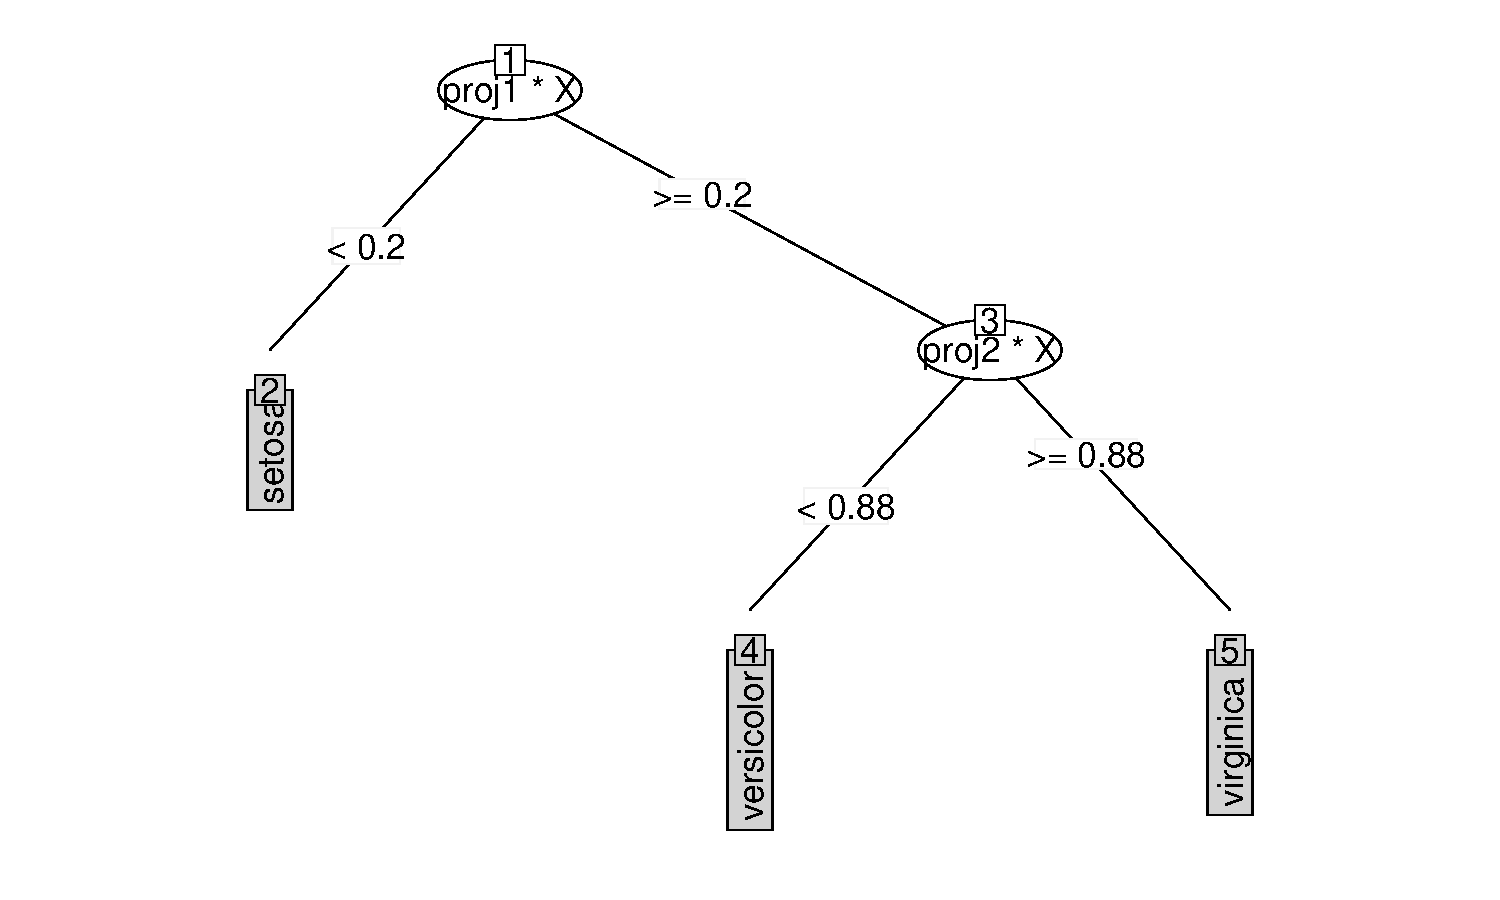
\includegraphics[width=0.5\textwidth]{ODRF-plot-the-tree-structure-of-class-ODT}
		}
		%\end{minipage}
		%\begin{minipage}{0.48\linewidth}
		%\centering%\flushright %,height=6
		\subfloat[The tree structure of class party of ODT]{
			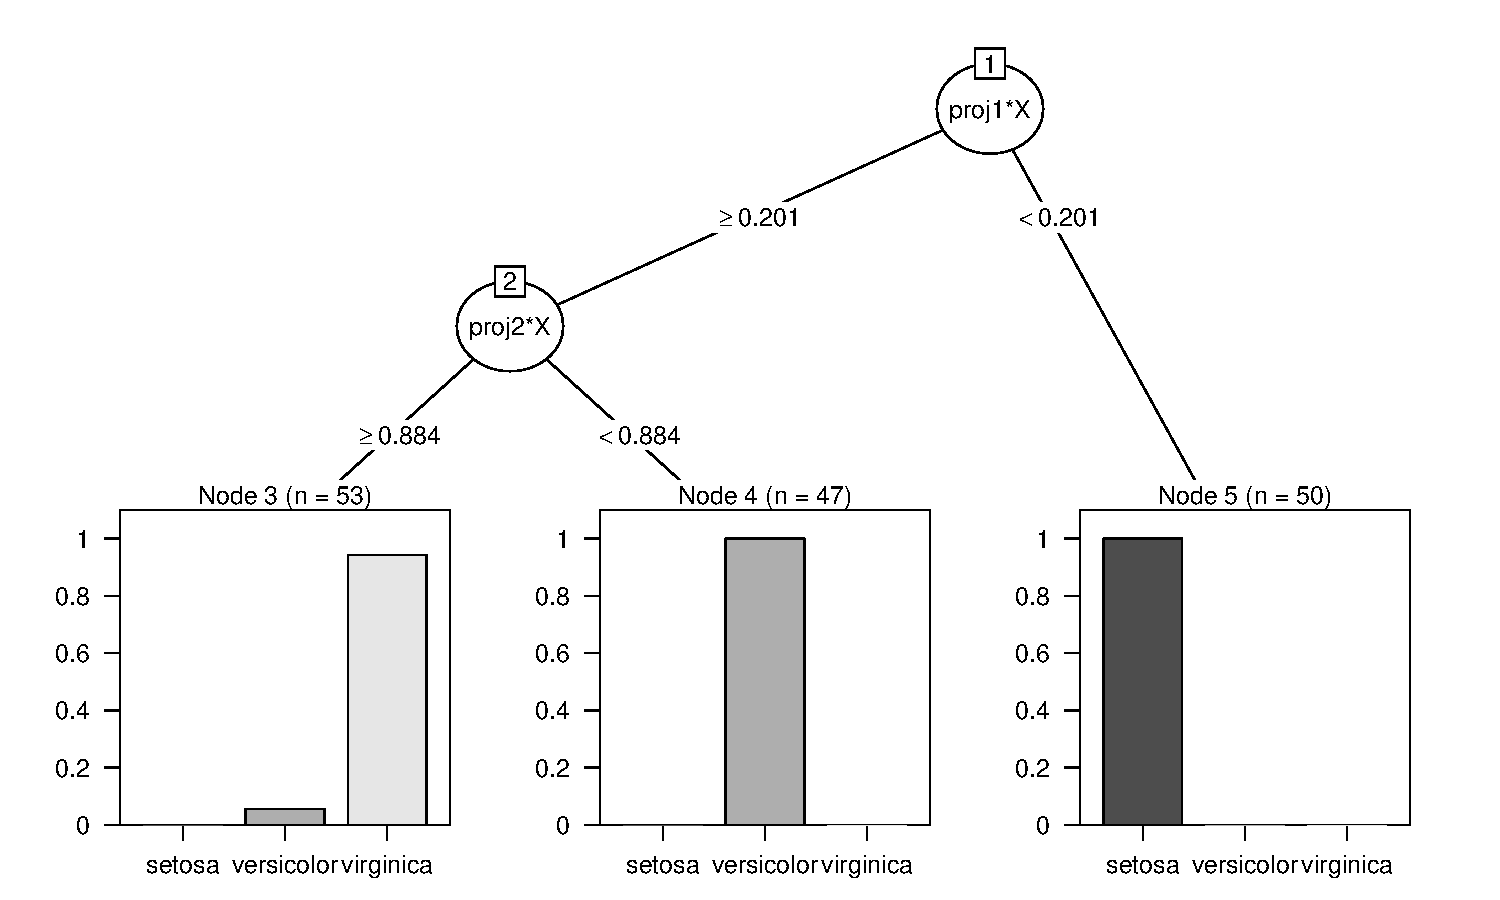
\includegraphics[width=0.5\textwidth]{ODRF-plot-the-tree-structure-of-class-part}
		}
		%\end{minipage}
		\caption{\label{fig:tree.structure}Two types of the tree structure.}
	\end{figure}
Below is one example, while the two types of tree plots are shown in  Figure~\ref{fig:tree.structure}.
\begin{example}
set.seed(0308)
tree <- ODT(Species ~ ., data = iris, split = "gini")
plot(tree, main = "")
party.tree <- as.party(tree, data = iris)
plot(party.tree)
\end{example}

For \fct{ODRF}, we provide functions \fct{Accuracy} to calculate the fitting accuracy and \fct{plot.Accuracy} to plot the fitting errors. Hereafter, we refer to errors as misclassification rate (MR) for classification or mean squared error (MSE) for regression.
Functions \fct{VarImp} and \fct{plot.VarImp} measure the variable importance and plot the dotchart of variable importance, respectively, where the variable importance is similarly calculated as \fct{importance} in \CRANpkg{randomForest} package.
{Our implementation uses impurity-based and permutation-based methods to measure the variable importance. It should be emphasized that our impurity-based method inherently incorporates these projection coefficients into the importance ranking. Specifically, for each splitting node, we randomly select $q$ projection variables from the $p$ predictor variables and define the variable importance measure as:
$$V_k = D \cdot \left| Q_k \right|, \quad k = j_1, j_2, \cdots, j_q$$
where $D$ represents the total decrease in node impurities from splitting on the variable, and $Q_k$ denotes the coefficient of the $k$-th projection. Consequently, $V_k$ constitutes a comprehensive metric for variable importance that integrates both impurity reduction and projection coefficient information. 
}
\begin{example} 
## S3 method for class 'VarImp'
varimp = VarImp(obj, X, y)
plot(varimp, nvar, digits = NULL, ...)

## S3 method for class 'Accuracy'
accuracy = Accuracy(obj, data, newdata = NULL)
plot(accuracy, lty = 1, digits = NULL, main = NULL, ...)
\end{example}
Below is an example. 
%
%Plot the error graph and dotchart of variable importance with respect to ODRF as Figure~\ref{fig:forest.error}.
%
\begin{example}
set.seed(3)
data(breast_cancer, package = "ODRF")
train <- sample(1:569, 300)
train_data <- breast_cancer[train, -1]
test_data <- breast_cancer[-train, -1]
forest <- ODRF(diagnosis ~ ., train_data,split = "gini", parallel = FALSE)
error <- Accuracy(forest, train_data, test_data)
plot(error)
varimp <- VarImp(forest, train_data[, -1], train_data[, 1])
plot(varimp, nvar = 10)
\end{example}
\begin{figure}[h!]
	\centering
	\centering
	\subfloat[Fitting errors of ODRF.]{
		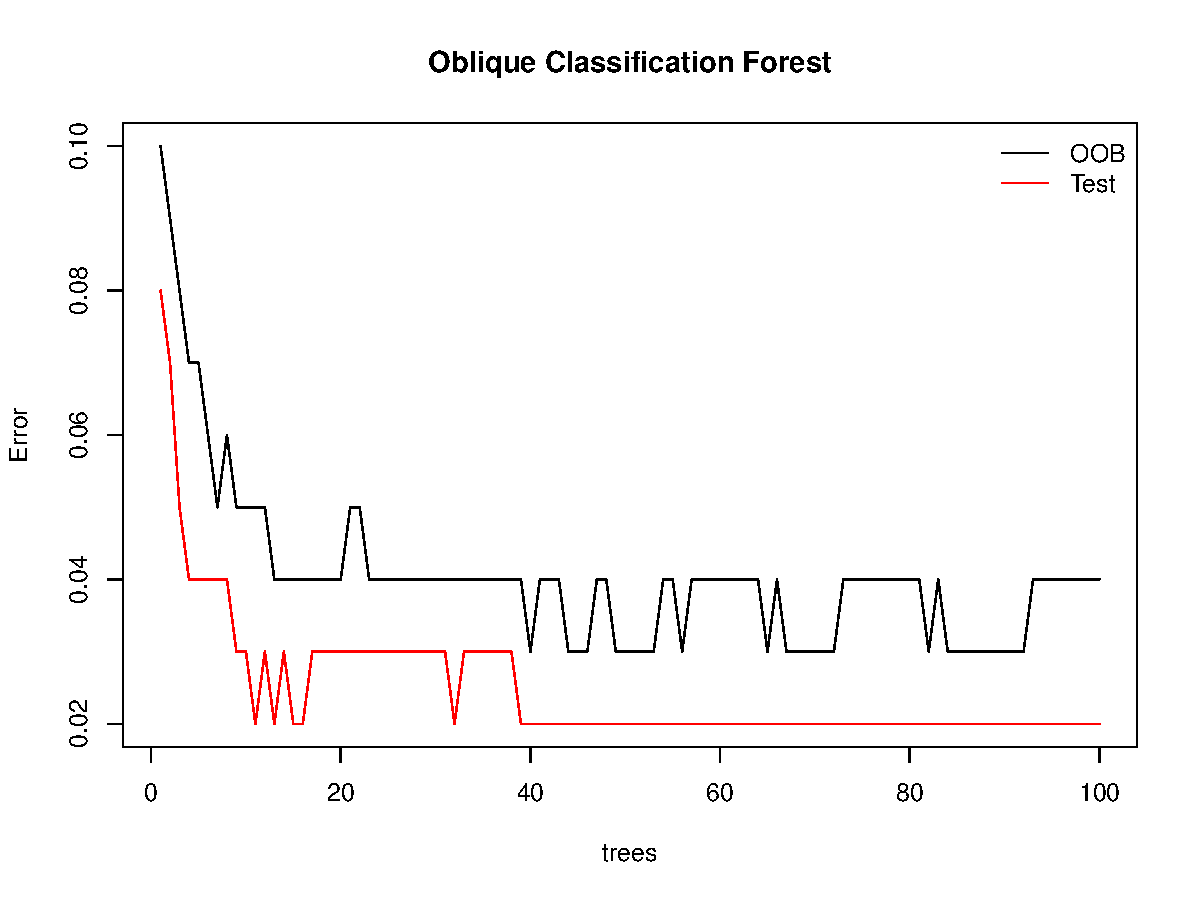
\includegraphics[width=0.45\textwidth]{ODRF-plot-the-error-graph-of-ODRF}
	}
	\subfloat[Dotchart of variable's importance.]{
		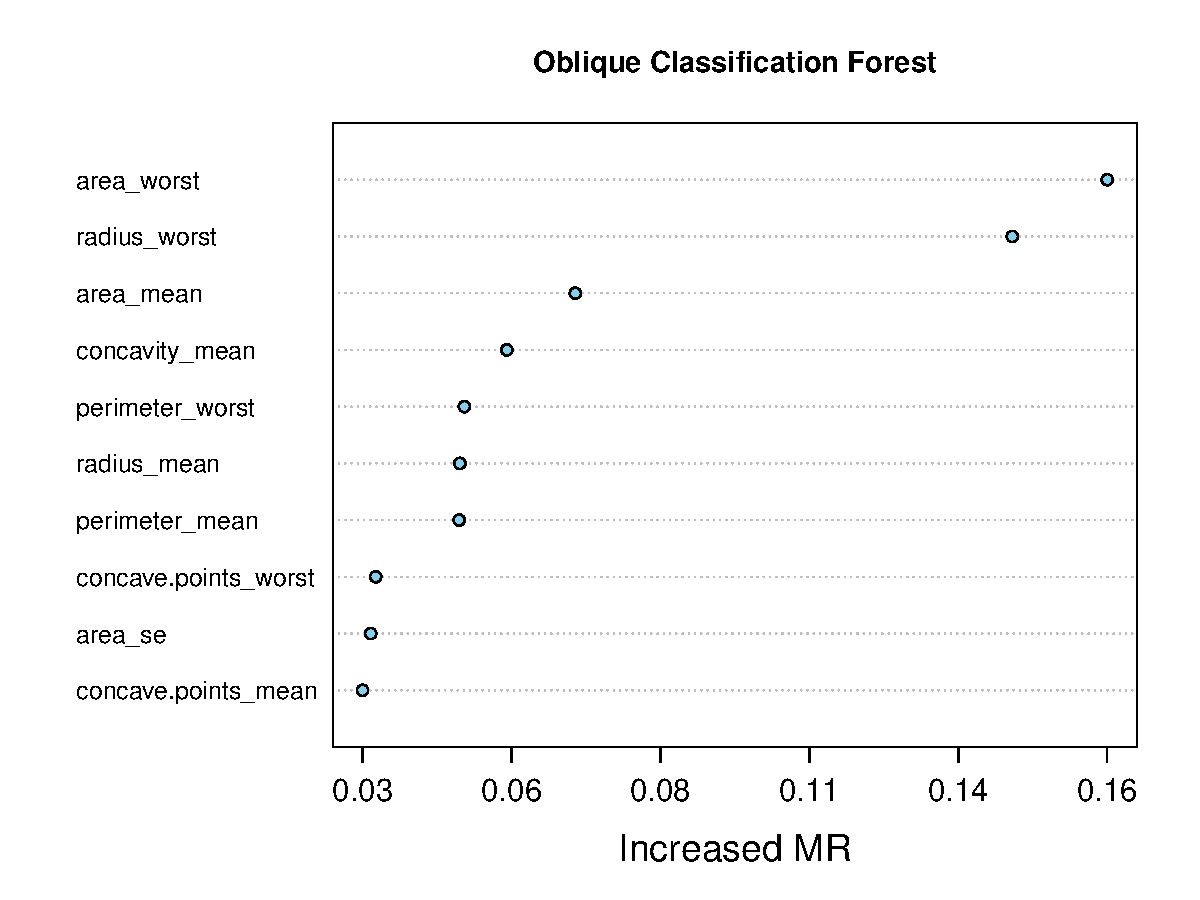
\includegraphics[width=0.45\textwidth]{ODRF-plot-the-dotchart-of-variable-importance-about-ODRF}
	}
	\caption{\label{fig:forest.error} The error of ODRF for classification and variable's importance.}
\end{figure}
The plots are shown in Figure~\ref{fig:forest.error}. The left panel is the plot of errors of ODRF against the number of trees. It can be seen that the errors of OOB and test data decrease with the number of trees and that the error of test data is bigger than the training data. The right panel is the dotchart of variable importance, the horizontal axis is the error of ODRF after removing one variable; the larger the error increases, the more important the variable is.

\subsection[Create a rotation matrix with RotMat* and user-defined functions]{Create a rotation matrix with \code{RotMat*} and custom functions} \label{user-defined}

\CRANpkg{ODRF} provides many ways to select the rotation directions $ \theta $ in each nodes, including  \fct{RotMatPPO}, \fct{RotMatRand} and \fct{RotMatRF}. The generated rotation matrix has three columns, the first column (\code{Variable}) is variables to be projected, the second column (\code{Number}) is the index of a projection, and the third column (\code{Coefficient}) is the coefficient of the projection for the variable. Details can be found by \code{?ODT} and \code{?ODRF}. %In addition, the user can define a projection matrix function, see the \CRANpkg{ODRF} help file for more details on usage.

The default method for the projection of \fct{RotMatPPO} is \code{model = "PPR"}, projection pursuit regression from \fct{ppr} in \code{stats} package  \citep{friedman1981projection}. %When response $y$ is a category label, it is expanded to $K$ binary features.
Standard usage is as follows.
\begin{example}
RotMatPPO(X, y, model = "PPR", dimProj, numProj, ...)
RotMatMake(X = NULL,y = NULL,RotMatFun = "RotMatPPO",PPFun = "PPO", ...)
\end{example}
%RotMatPPO(X, y, dimProj = 3, numProj = 2, model = "PPR", split = "mse")
Here is one example.
\begin{example}
set.seed(14)
X <- matrix(rnorm(1000), 200, 5)
y <- (X[,1]+X[,2])^2 + X[,4]-X[,5] +  runif(200)
tree <- ODT(X, y, split = "mse", NodeRotateFun = "RotMatPPO",
  paramList = list(model = "PPR", dimProj = 5, numProj = 1))
round(tree[["projections"]],2)
\end{example}
\begin{example}
         X1    X2    X3   X4    X5
proj1  0.20  0.29 -0.09 0.63 -0.69
proj2 -0.69 -0.68  0.02 0.19 -0.16
proj3 -0.06 -0.09  0.16 0.72 -0.67
proj4 -0.57 -0.70  0.03 0.31 -0.29
\end{example}
It can be seen that  the projections are roughly parallel to those in the model, i.e. (1, 1, 0, 0, 0) and (0, 0, 0, 1, -1).  

It is worth mentioning that the package allows users to  define their rotation matrix functions and link them with the function \fct{RotMatMake} in the package.  The first function, named, for example, \fct{makeRotMat}, is to select  the variables to be projected, with a specified format of  output, including the projection dimensions and the number of projections (the first two columns of the rotation matrix): 
\begin{example}
makeRotMat <- function(dimX, dimProj, numProj, ...) {
  RotMat <- matrix(1, dimProj * numProj, 3)
  for (np in seq(numProj)) {
    RotMat[(dimProj * (np - 1) + 1):(dimProj * np), 1] <-
    sample(1:dimX, dimProj, replace = FALSE)
    RotMat[(dimProj * (np - 1) + 1):(dimProj * np), 2] <- np
    RotMat[(dimProj * (np - 1) + 1):(dimProj * np), 3] <- 
    sample(c(1L, -1L), dimProj, replace = TRUE, prob = c(0.5, 0.5))
  }
  return(RotMat)
}
set.seed(35)
RotMat1 <- makeRotMat(dimX = 5, dimProj = 3, numProj = 2)
RotMat1
\end{example}
\begin{example}
     [,1] [,2] [,3]
[1,]    2    1   -1
[2,]    5    1   -1
[3,]    1    1   -1
[4,]    5    2    1
[5,]    2    2    1
[6,]    4    2   -1
\end{example}
The second  function, named as, for example, \fct{makePP}, is defined to estimate  the projection coefficients (the third column of the rotation matrix):
\begin{example}
makePP <- function(X, y, ...) {
  LM <- lm(y ~ ., data = data.frame(X,y=y))
  theta <- as.matrix(LM[["coefficients"]])[-1, , drop = FALSE]
  theta <- theta / sqrt(sum(theta^2))
  return(theta)
}
set.seed(35)
RotMat3 <- RotMatMake(X = X, y = y, RotMatFun = "makeRotMat", PPFun = "makePP", 
  paramList = list(dimX = 5, dimProj = 3, numProj = 2))
RotMat3
\end{example}
\begin{example}
     Variable Number Coefficient
[1,]        2      1   0.4297059
[2,]        5      1  -0.9007557
[3,]        1      1   0.0631821
[4,]        5      2  -0.7227304
[5,]        2      2   0.2141932
[6,]        4      2   0.6571012
\end{example}
Then, we put these functions as augments of \code{NodeRotateFun} and \code{PPFun} respectively as follows.
%
%Train ODT with defined functions \fct{makeRotMat} and \fct{makePP}.
%
\begin{example}
set.seed(23)
tree <- ODT(X, y, split = "mse", NodeRotateFun = "RotMatMake", paramList = 
  list(RotMatFun = "makeRotMat", PPFun = "makePP", dimX = 5, dimProj = 5, numProj = 1))
round(tree[["projections"]], 2)
\end{example}
\begin{example}
         X1    X2    X3   X4    X5
proj1  0.08  0.21 -0.11 0.69 -0.68
proj2  0.22  0.39 -0.16 0.69 -0.55
proj3 -0.27 -0.03  0.05 0.68 -0.68
\end{example}

\section{Real examples} \label{sec:examples}

In this section, we first use \fct{ODT} to analyze two data sets and see how it improves the analysis of CART,  in terms of  model complexity, model fitting and variable importance. In the second example, we compare the prediction performance of ODT and ODRF in \CRANpkg{ODRF} with the other popular methods using 43 real data sets, including 20 continuous responses, 8 multinomial responses and 15 binary responses. All real data analyses were conducted in R version 4.2.2 on a Windows 11 Operating System with AMD Ryzen 7 5800H with Radeon Graphics (16 CPUs), ~3.2~GHz with 16~GB of memory.
%half of which have continuous responses and the other half categorical.
%In addition, we add the forest methods and consider the time consumption and tree complexity. The rest of the section describes how to use our ODRF package in real data, and we explain the use of two data sets with continuous and categorical response.

\subsection{Two data sets for complexity analysis}

The first dataset is the kyphosis data, which has 81 observations. The data (\code{kyphosis}) are available at \CRANpkg{rpart}.  The response is $kyphosis$ with values  'absent' or 'present', indicating whether kyphosis (a type of deformity) was present after surgery. The three predictors are (1) $age$: the age of the child in months; (2) $number$: the number of vertebrae involved; (3) $start$: the number of the first (uppermost) vertebra operated on.  Below is the code and analysis. 
%The data was obtained from the \CRANpkg{rpart} package by \code{data(kyphosis,package = "rpart")}, and the key challenges against it's detection is how to classify kyphosis into absent or present. We first 
%Fit error of kyphosis.
%
%
%The trees of ODT and CART are shown in Figure \ref{fig:tree of kyphosis}.
%
\begin{figure}[h!]
	\centering
	\centering
	\subfloat[The ODT tree structure of kyphosis.]{
		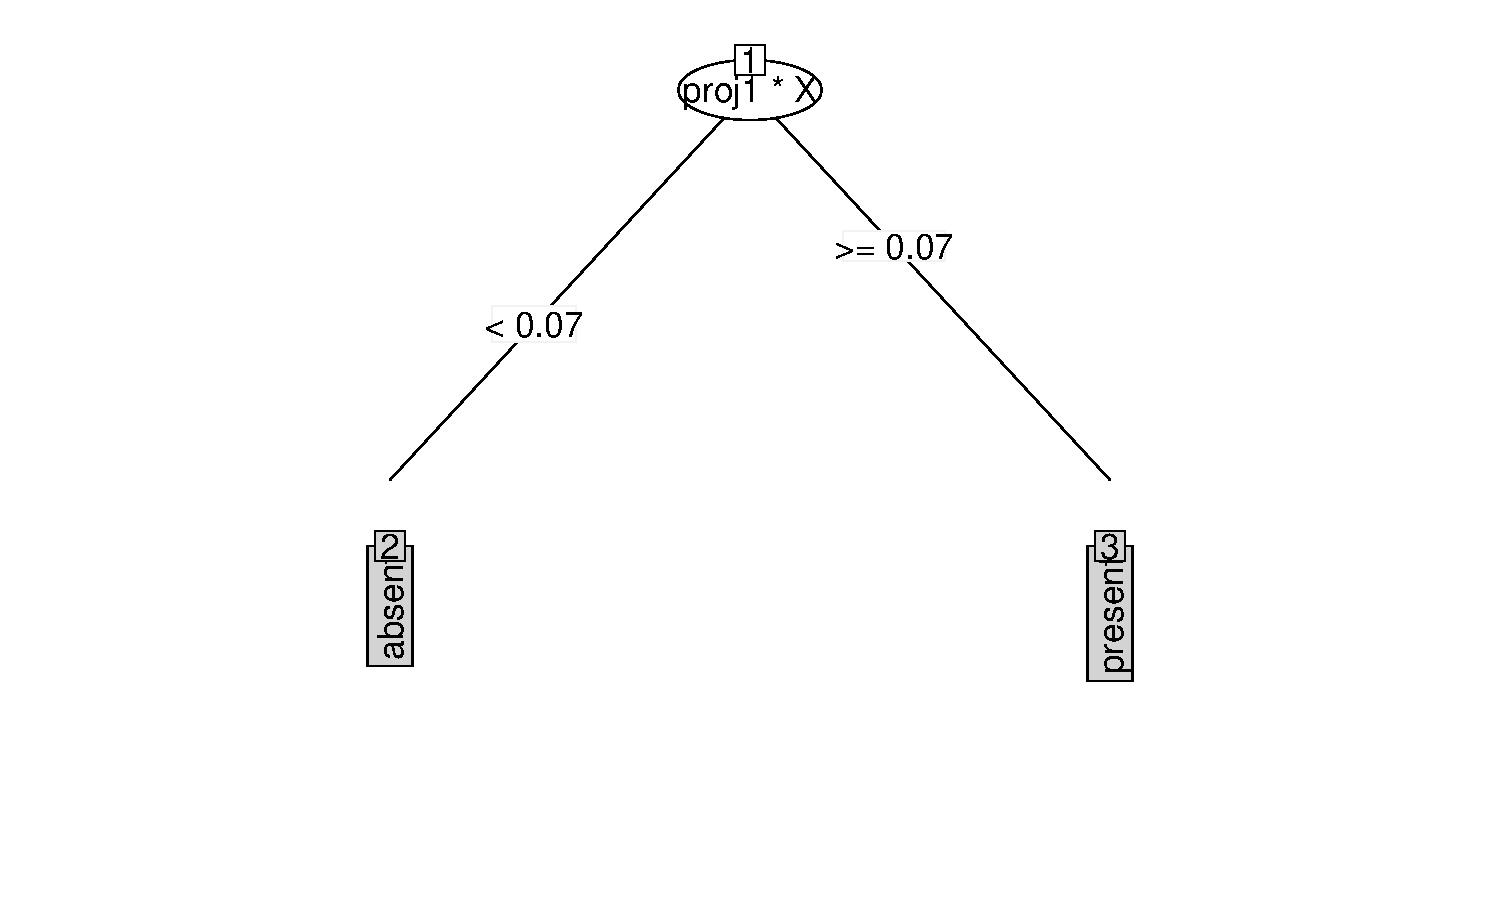
\includegraphics[width=0.5\textwidth]{ODRF-The-ODT-tree-structure-of-kyphosis}
	}
	\subfloat[The \CRANpkg{rpart} tree structure of kyphosis.]{
		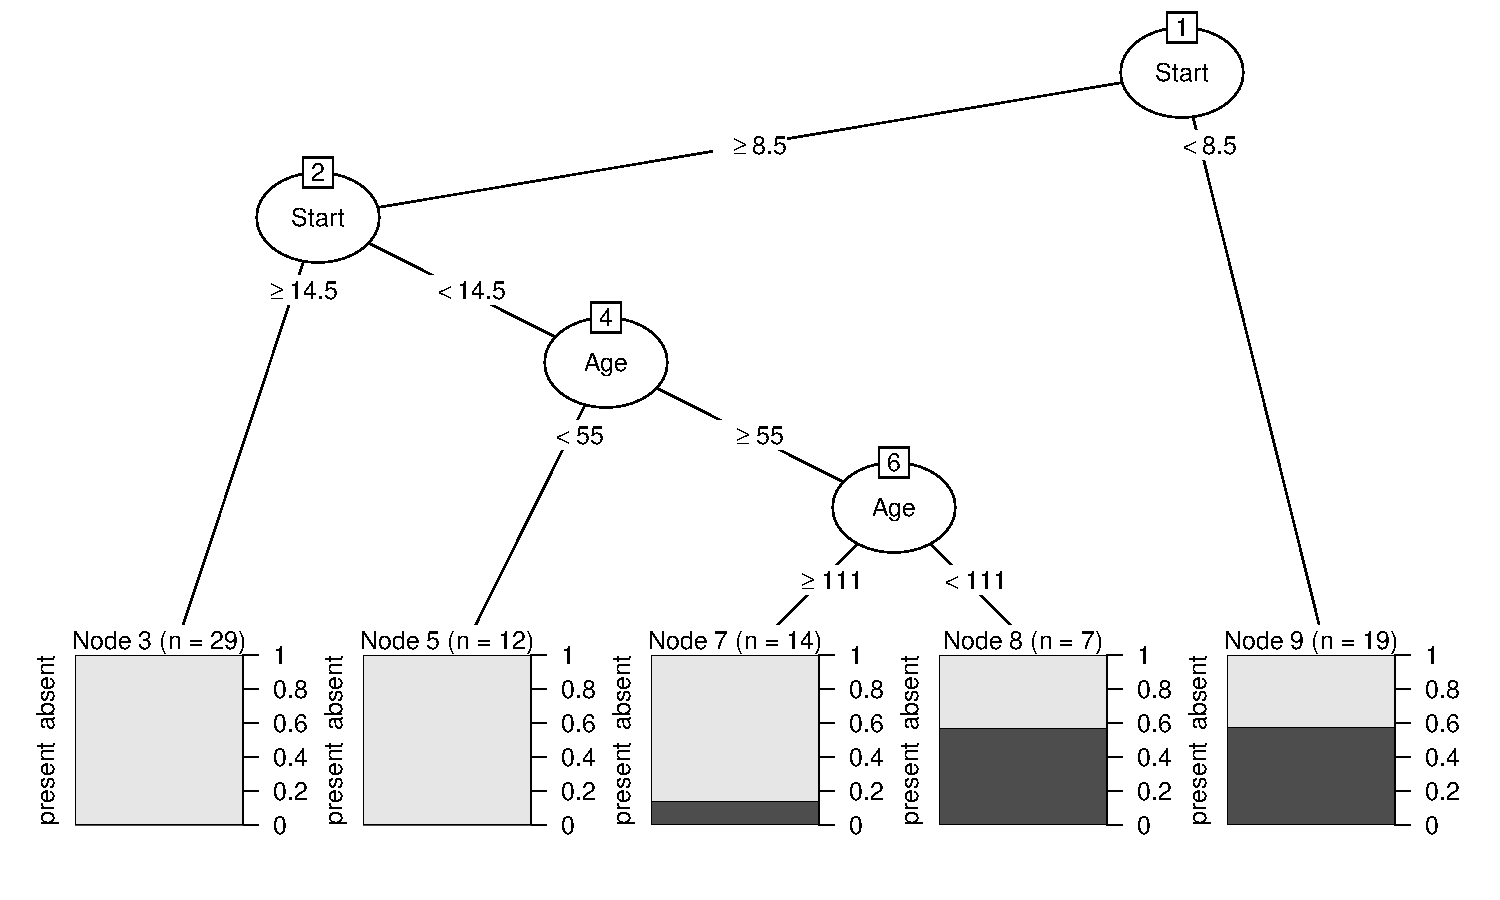
\includegraphics[width=0.5\textwidth]{ODRF-The-rpart-tree-structure-of-kyphosis}
	}
	\caption{\label{fig:tree of kyphosis} The tree structure of kyphosis of ODT and the conventional CART respectively.}
\end{figure}
We first fit the data to ODT and CART, and calculate the fitted errors.   
\begin{example}
data(kyphosis, package = "rpart")
odt <- ODT(Kyphosis ~ Age + Number + Start, data = kyphosis, split = "gini", 
  paramList = list(model = "PPR", numProj = 1))
tree <- rpart(Kyphosis ~ Age + Number + Start, data = kyphosis, method = "class")
pred <- predict(odt, kyphosis[, -1])
e.odt <- mean(pred != kyphosis[, 1])
pred <- predict(tree, kyphosis, type = "class")
e.tree <- mean(pred != kyphosis[, 1])
print(c(e.odt = e.odt, e.tree = e.tree))
\end{example}
\begin{example}
    e.ODT    e.CART 
0.1604938 0.1604938
\end{example}
\begin{example}
print(round(odt[["projections"]], 3))
\end{example}
\begin{example}
       Age Number  Start
proj1 0.31  0.596 -0.741
\end{example}
The trees of ODT and CART are shown in Figure \ref{fig:tree of kyphosis}. We can see from the trees that ODT has a much smaller complexity, i.e.~2 leaves, than CART which has 5 leaves,  but has the same fitted error as CART. There is only one projection for ODT with splitting variable $ 0.310 \times \text{Age} + 0.596 \times \text{Number} - 0.74 \times \text{Start} $, which determines whether kyphosis will present or not after an operation. 

The second data set is about the relative performance and characteristics of 209 CPUs. This dataset contains the following variables: $syct$  (cycle time in nanoseconds), $mmin$ (minimum main memory in kilobytes),  $mmax$ (maximum main memory in kilobytes),  $catch$ (cache size in kilobytes),  $chmin$ ( minimum number of channels), $chmax$ (maximum number of channels),   $perf$ (published performance on a benchmark mix relative to an IBM 370/158-3), and  $estperf$ (estimated performance by Ein-Dor \& Feldmesser). This data (\code{cpus}) is available in \CRANpkg{MASS}. The interest is to predict the $perf$ using $syct$, $mmin$, $mmax$, $cach$, $chmin$ and $chmax$. The logarithm transformation is made to $perf$.
\begin{figure}[h!]
	\centering%height=5.5,
	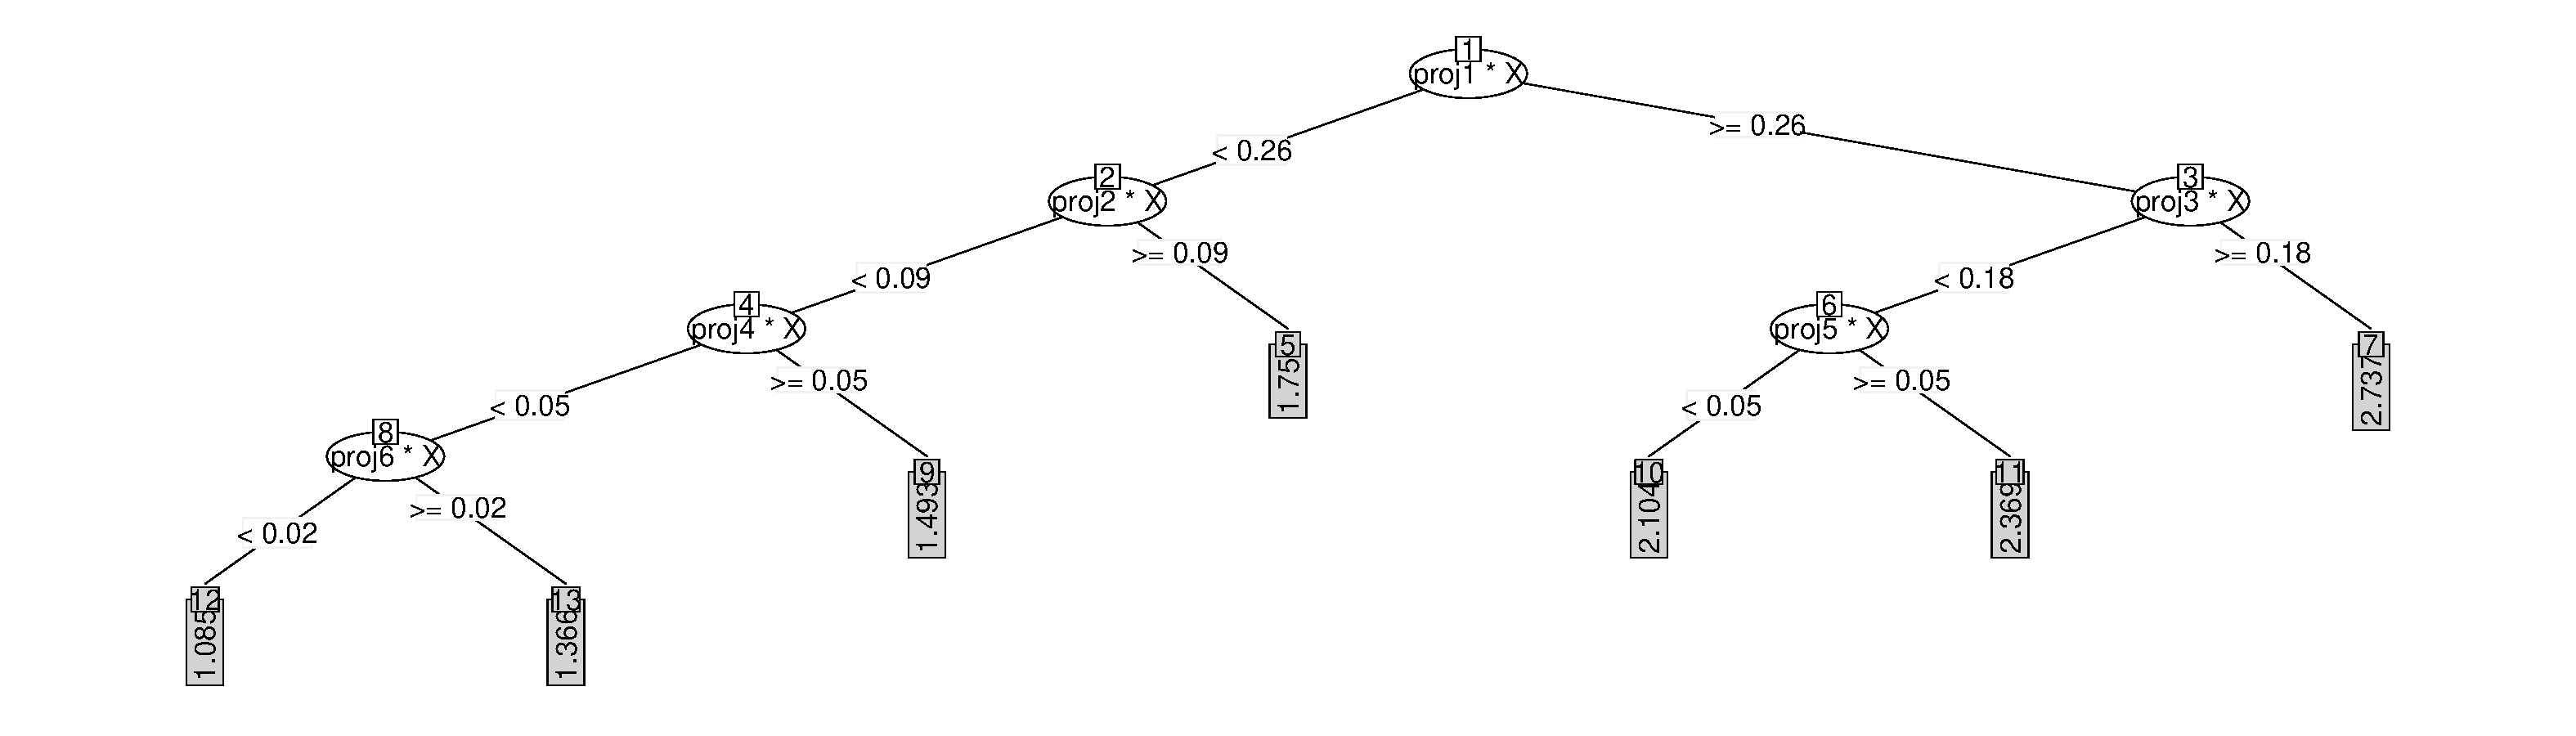
\includegraphics[width=\textwidth]{ODRF-The-ODT-tree-structure-of-cpus}
	\caption{\label{fig:ODT of cpus}  ODT tree structure of cpus}
\end{figure}

\begin{example}
data(cpus, package = "MASS")
odt <- ODT(log10(perf) ~ syct + mmin + mmax + cach + chmin + chmax, data = cpus, 
  lambda = log(nrow(cpus)), split = "mse", paramList = list(model = "PPR", numProj = 1))
pred <- predict(odt, cpus[, 2:7])
e.odt <- mean((pred - log10(cpus[, 8]))^2)
tree <- rpart(log10(perf) ~ syct + mmin + mmax + cach + chmin + chmax,   data = cpus)
pred <- predict(tree, cpus)
e.tree <- mean((pred - log10(cpus[, 8]))^2)
print(c(e.ODT = e.odt, e.CART = e.tree))
\end{example}
\begin{example}
     e.ODT     e.CART 
0.02297886 0.03034244 
\end{example}
\begin{example}
print(round(odt[["projections"]], 3))
\end{example}
\begin{example}
	syct   mmin  mmax   cach chmin  chmax
proj1 -0.047  0.546 0.586  0.553 0.206  0.094
proj2 -0.021  0.298 0.505  0.744 0.319  0.014
proj3 -0.963  0.125 0.181  0.121 0.010  0.101
proj4 -0.034  0.751 0.419  0.407 0.302  0.051
proj5 -0.982 -0.002 0.126  0.070 0.000  0.125
proj6 -0.012 -0.351 0.920 -0.156 0.061 -0.049
\end{example}
The ODT and CART trees are depicted in Figure \ref{fig:ODT of cpus} and Figure \ref{fig:rpart of cpus}, respectively. Once again, it is evident that ODT has fewer leaves and a lower fitting error than CART. Interestingly, the first, second, and fourth projections primarily relate to a computer's memory and the time required to fetch data from main memory or disk storage (represented by $mmin$, $mmax$, $catch$, $chmin$), as their coefficients have larger absolute values. Another group of projections, specifically the third and fifth, are associated with $syct$, the time it takes a computer to complete one clock cycle, which can contribute to faster processing speeds and improved performance.
In some special cases, $mmax$ plays a role, i.e.~projection~6, possibly when the data set is large. These projections correspond to the common understanding of the performance of a computer and its hardware settings. These examples show that ODT has better interpretability than CART. 
\begin{figure}[h!]
	\centering
	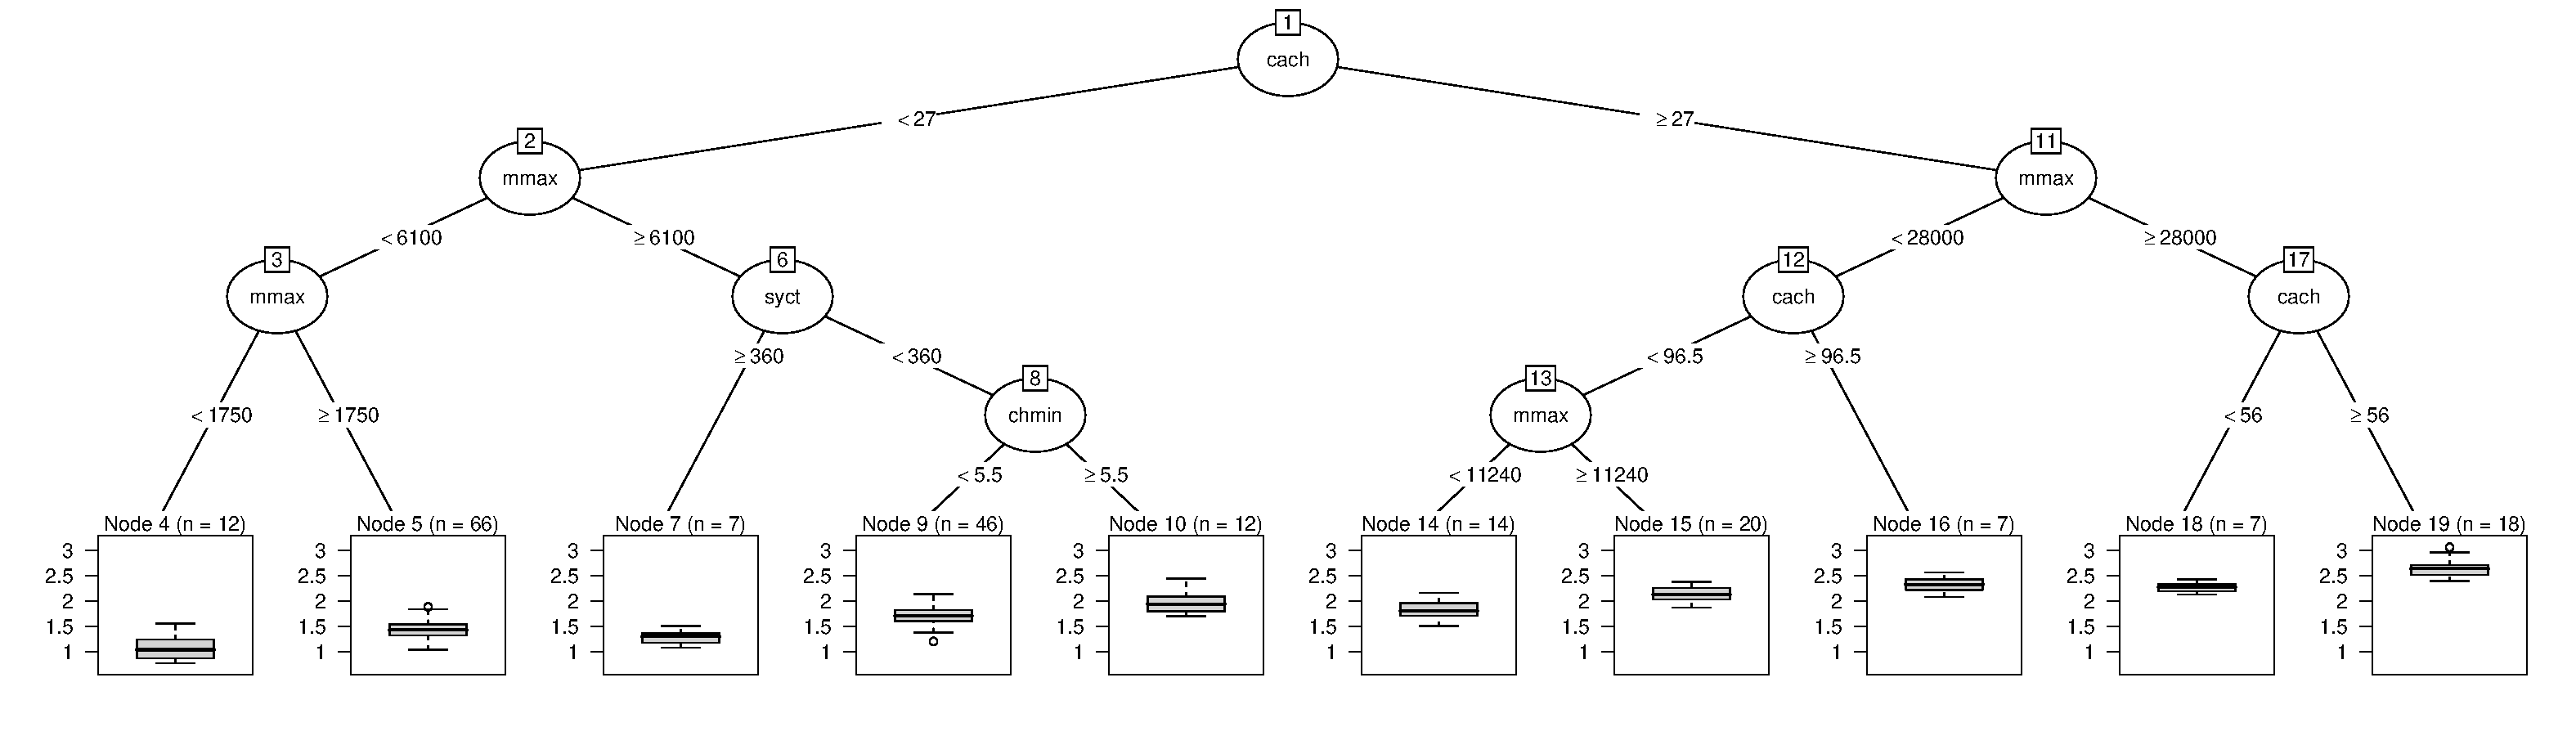
\includegraphics[width=\textwidth]{ODRF-The-rpart-tree-structure-of-cpus.pdf}
	\caption{\label{fig:rpart of cpus} The conventional  tree structure of cpus using  \CRANpkg{rpart}.}
\end{figure}

%
%Plot the importance of variables for mtcars.
%
\begin{figure}[h!]
	\centering
	%\subfloat[]{
		%\begin{minipage}{0.48\linewidth}height=0.2\textheight
		\centering%\flushleft %,,height=6,height=0.2\textheight
		\subfloat[LASSO]{
			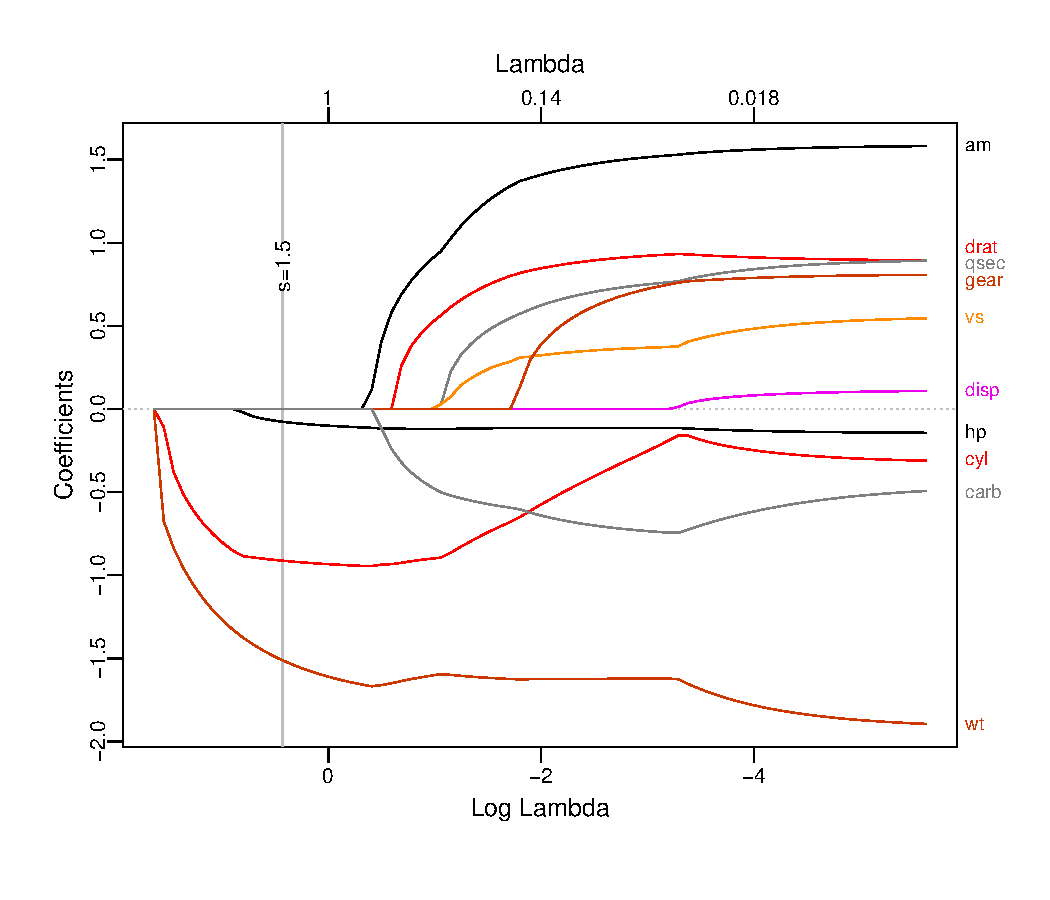
\includegraphics[width=0.3\textwidth]{ODRF-plot-the-importance-of-variables-for-mtcars-with-LASSO}
		}
		%\end{minipage}
		%\begin{minipage}{0.48\linewidth}
		%\centering%\flushright %,height=6
		\subfloat[RF]{

			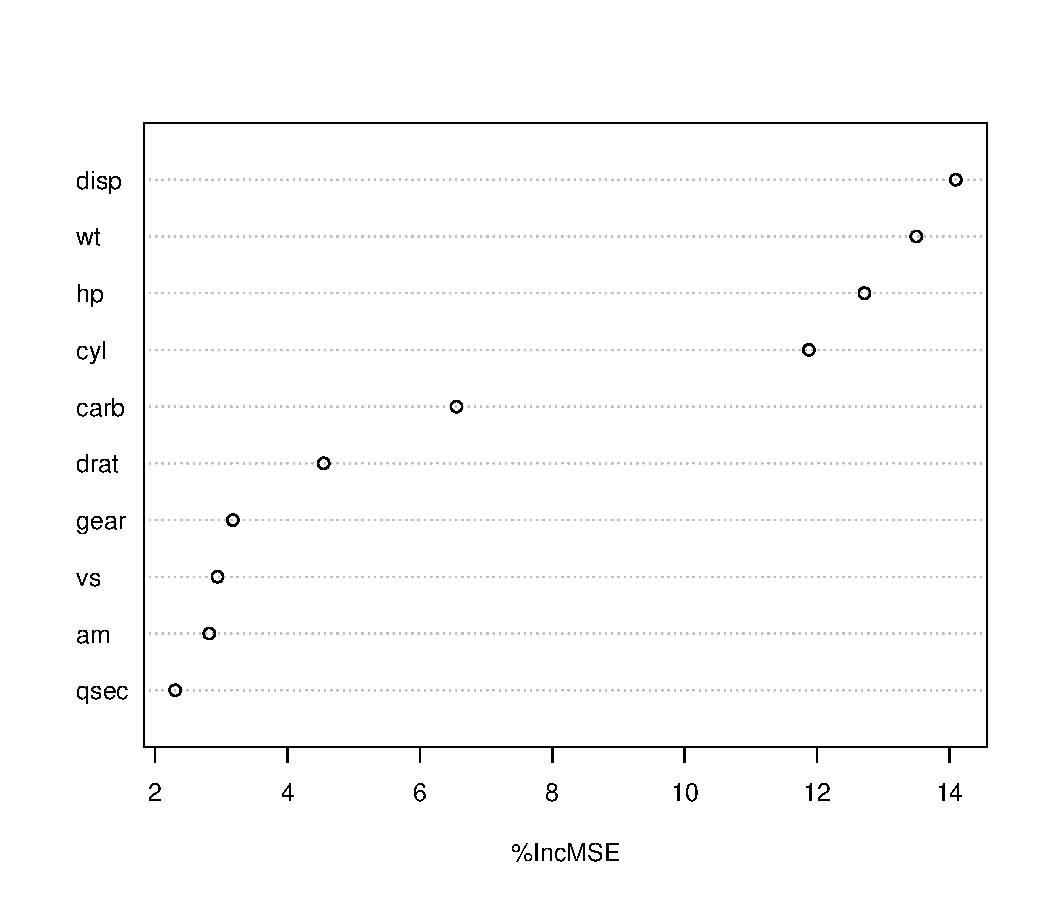
\includegraphics[width=0.3\textwidth]{ODRF-plot-the-importance-of-variables-for-mtcars-with-RF}
		}
		\subfloat[ODRF]{
			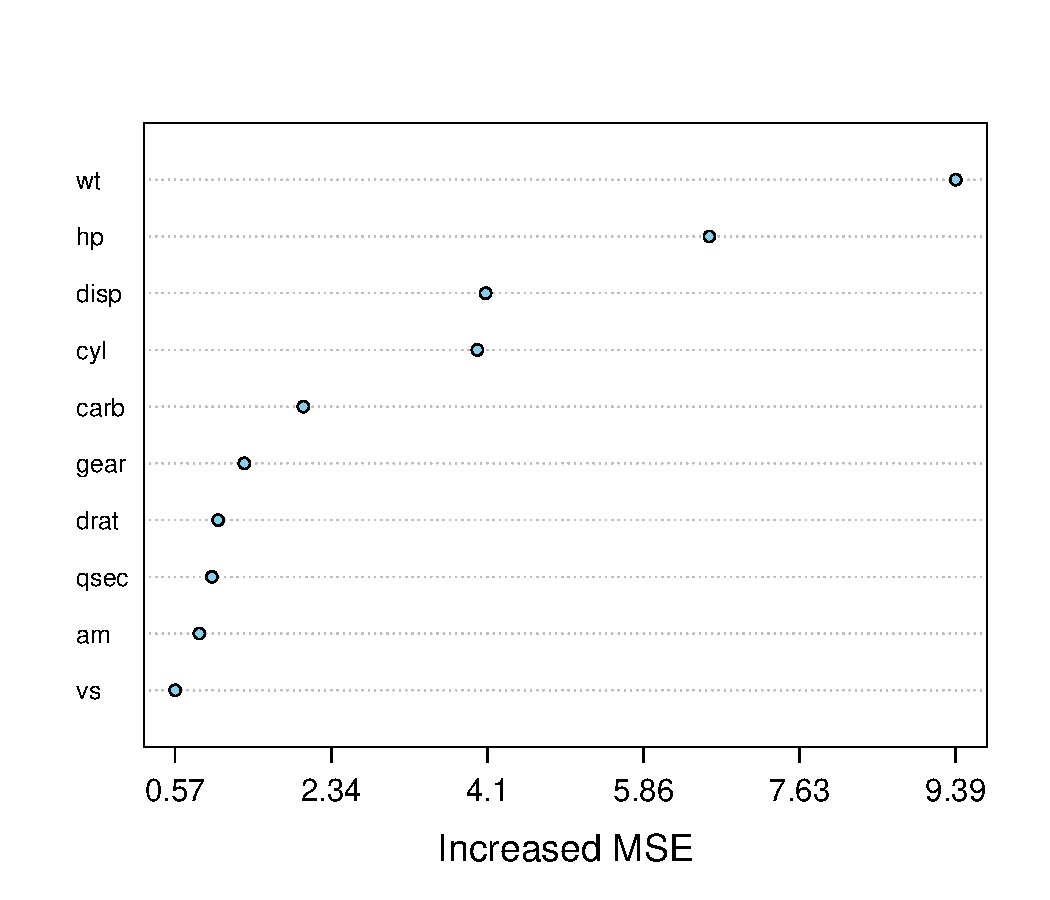
\includegraphics[width=0.3\textwidth]{ODRF-plot-the-importance-of-variables-for-mtcars-with-ODRF}
		}
		%\end{minipage}
		\caption{\label{fig:var.imp.mtcars} Plots of the importance of variables for data ``mtcars'' using three methods.}
	\end{figure}
\subsection{Analysis  of the importance of variables}

The data was extracted from the 1974 Motor Trend US magazine, and comprises fuel consumption and 10 aspects of automobile design, including mpg: Miles/(US) gallon, cyl: Number of cylinders, disp: Displacement (cu.in.), hp: Gross horsepower, drat: Rear axle ratio, wt: Weight (1000 lbs), qsec: 1/4 mile time, vs: Engine (0 = V-shaped, 1 = straight), am: Transmission (0 = automatic, 1 = manual), gear: Number of forward gears, and carb: Number of carburetors, and performance, which is measured by the fuel consumption (mpg).  This data (\code{mtcars}) is available in \code{datasets} \citep{henderson1981building}. Our interest is to explore which aspects of automotive design affect the performance (mpg).

ODRF measures variable importance using a similar permutation method as RF. We will compare the rank of importance of ODRF with RF. In addition, LASSO is a popular variable selection method, so we use it as a benchmark. Figure~\ref{fig:var.imp.mtcars} shows that ODRF ranks Weight (wt) as the most important factor affecting fuel consumption, which is consistent with the LASSO results. RF ranks Displacement (disp) as an important influencing factor, while the LASSO results show Displacement as the least influencing factor. Further comparison of the other variable rankings shows that our ODRF rankings of variable importance are generally consistent with LASSO, while RF differs more.

\begin{table}[h!]
	\centering
	%\begin{center}
	\begin{minipage}{\textwidth}
		\setlength{\tabcolsep}{0.6mm}{
			\begin{tabular}{@{\extracolsep{\fill}}lrrcccccccc@{\extracolsep{\fill}}}%{lrrrrrrrrr}% {\textwidth}{@{\extracolsep{\fill}}lrrrrrrrrr@{\extracolsep{\fill}}}%{lrrrrrrrrr{7.4cm}}%
				%\multirow{2}[4]{*}{Dataset} & \multirow{2}[4]{*}{n} & \multirow{2}[4]{*}{p} & \multicolumn{4}{c}{Axis-aligned} & \multicolumn{3}{c}{Oblique} \\
				%\cmidrule{4-10}          &       &       & CART  & ERT   & EVT   & CT    & rotT  & SPOT  & ODT \\
				\toprule%
				&       &         & \multicolumn{4}{c}{Axis-aligned} & \multicolumn{4}{c}{Oblique} \\
				%\cline{4-7} \cline{8-10}
				\cmidrule(lr){4-7}\cmidrule(lr){8-11}%
				Dataset&   n    &   p      & CART  & ERT   & EVT   & CT    & RotT  & SPOT &PPT & ODT \\
				\midrule
				Servo (C)  & 166   & 4     & 0.298  & 0.812  & \pmb{0.257}& 0.300  & 0.770  & 0.563  &0.387 & 0.306  \\
				AutoMpg (C)  & 391   & 7     & 0.213  & 0.314  & 0.217  & 0.192  & 0.281  & 0.245 &0.184 & \pmb{0.175}\\
				Concrete Compressive (A) & 1030  & 8     & 0.314  & 0.513  & 0.308  & 0.248  & 0.539  & 0.446  &0.502& \pmb{0.202}\\
				Boston house price (A)  & 506   & 13    & 0.275  & 0.458  & 0.294  & 0.275  & 0.439  & 0.379 &0.262 & \pmb{0.261}\\
				Wild blueberry yield (B) & 777   & 13    & 0.228  & 0.347  & 0.224  & 0.189  & 0.319  & 0.265  & \pmb{0.099}&0.113\\
				Body fat (B) & 252   & 14    & 0.073  & 0.418  & 0.085  & \pmb{0.061}& 0.446  & 0.402  &0.096& 0.072  \\
				Paris housing price (B) & 10000 & 16    & 0.021  & 0.370  & 0.005  & \pmb{0.000}& 0.761  & 0.662  &0.006 & \pmb{0.000}\\
				House sales in King County (B) & 21613 & 18    & 0.327  & 0.482  & 0.324  & 0.287  & 0.442  & 0.360  &0.314& \pmb{0.256}\\
				Bar crawl (B) & 7590  & 21    & 0.323  & 0.498  & 0.326  & 0.297  & 0.499  & 0.429  & 0.326&\pmb{0.280}\\
				Auto 93 (C)  & 81    & 22    & 0.620  & 0.927  & 0.706  & 0.602  & 0.753  & 0.683  & 0.707&\pmb{0.599}\\
				Auto horsepower (C)  & 159   & 24    & 0.236  & 0.340  & 0.255  & 0.238  & 0.487  & 0.384  & 0.230&\pmb{0.189}\\
				Facebook comment volume (A) & 18370 & 52    & \pmb{0.700}& 1.210  & 0.756  & 0.717  & 0.971  & 0.846  &0.841 & 0.743  \\
				Gold price prediction (B) & 1718  & 74    & 0.043  & 0.023  & 0.023  & 0.016  & 0.136  & 0.029  &0.027& \pmb{0.010}\\
				Baseball player statistics (B) & 4535  & 74    & 0.039  & 0.225  & 0.017  & 0.010  & 0.646  & 0.470  &0.054& \pmb{0.007}\\
				CNNpred (A) & 1441  & 76    & 0.032  & 0.016  & 0.010  & 0.003  & 0.124  & 0.068  & 0.019&\pmb{0.002}\\
				Superconductivity (A) & 21263 & 81    & 0.296  & 0.387  & 0.293  & 0.287  & 0.332  & 0.309  & 0.323&\pmb{0.271}\\
				Warsaw flat rent price (B) & 3472  & 78    & 0.447  & 0.750  & 0.462  & \pmb{0.425}& 0.965  & 0.624  &0.518 & 0.469  \\
				Buzz in social media (A) & 28179 & 96    & 0.206  & 0.347  & 0.234  & \pmb{0.201}& 0.489  & 0.349  &0.378& 0.344  \\
				Communities and Crime (A) & 1994  & 101   & 0.475  & 0.746  & 0.480  & \pmb{0.445}& 0.568  & 0.526  &0.617& 0.545  \\
				Residential building-Sales (A) & 372   & 103   & 0.060  & 0.231  & 0.060  & \pmb{0.040}& 0.356  & 0.285 &0.176 & 0.046  \\
				\hline
				\multicolumn{3}{c}{Average RPE across all 20 datasets}&   0.261  & 0.471  & 0.267  & 0.242  & 0.516  & 0.416  &0.303& 0.245  \\
				\multicolumn{3}{c}{No.~of bests in 20 datasets} &
				1     & 0     & 1     & 6     & 0     & 0     &1 & 11 \\
				\bottomrule
		\end{tabular}}
	\end{minipage}
	%	\end{center}
\caption{Regression: average RPE based on 100 random partitions of each data set into training and test sets. The alphabetic notation in the brackets of each dataset represents the data source.}\label{Table1}%
\end{table}%

\subsection{Prediction performance}
%We follow the experimental design of \cite{zhan2022consistency}, where the performance of  \code{ODRF} was presented.

 Next, we show the performance of \code{ODT} and \code{ODRF} as well. We use 20 real data sets with continuous responses  and 23 data sets with categorical responses for regression and classification respectively.  Our data are mainly obtained from the UCI machine learning database (A) \url{https://archive.ics.uci.edu/ml/datasets}, the Kaggle database (B) \url{https://www.kaggle.com}, and  the Collection of Datasets of \cite{rainforth2015canonical} (C) \url{https://github.com/twgr/ccfs/}. All data can also be obtained directly from \url{https://github.com/liuyu-star/RJ_ODRF_Codes}.
If there are any missing values in the data, the corresponding observations are removed from the data. %In the calculation, each predictor is scaled to [0, 1] which is the default transformation of the package.
{ We scale the predictors individually before performing the calculation. Although this makes no theoretical difference, it sometimes enhances computational stability and facilitates variable importance ranking.}  

{
The estimation methods of the coefficients of these projections include random projection, logistic regression, dimension reduction and many others. However, our experiments suggest that these estimations actually make little difference in
the results. In our calculation, instead of using one single projection or linear combination, we provide
a number of projections, each of which is for the projection of a set of randomly selected predictors, and then use Gini impurity or residual sum of squares to choose one combination as splitting variable and splitting point. The logistic regression function is used to find projections for each combination of predictors, but other alternatives are also provided in the package.}

\begin{table}[h!]
	\centering
	%\begin{center}
	{ \small
		\begin{minipage}{\textwidth}
			\setlength{\tabcolsep}{0.8mm}{
				\begin{tabular}{@{\extracolsep{\fill}}lrrrrrrrrrrr@{\extracolsep{\fill}}}%{lrrrrrrrrr}% {\textwidth}{@{\extracolsep{\fill}}lrrrrrrrrr@{\extracolsep{\fill}}}%{lrrrrrrrrr{7.4cm}}%
					%\multirow{2}[4]{*}{Dataset} & \multirow{2}[4]{*}{n} & \multirow{2}[4]{*}{p} & \multicolumn{4}{c}{Axis-aligned} & \multicolumn{3}{c}{Oblique} \\
					%\cmidrule{4-10}          &       &       & CART  & ERT   & EVT   & CT    & rotT  & SPOT  & ODT \\
					\toprule%
					&       &         & \multicolumn{4}{c}{Axis-aligned} & \multicolumn{5}{c}{Oblique} \\
					%\cline{4-7} \cline{8-10}
					\cmidrule(lr){4-7}\cmidrule(lr){8-12}%
					Dataset&   n    &   p      & CART  & ERT   & EVT   & CT    & RotT  & SPOT  &PPT & OT & ODT \\
					\midrule
					Iris (A, 3) & 149   & 4     & 6.96  & 21.58  & 7.08  & 5.98  & 14.74  & 15.20  & \pmb{2.66} & 4.24  & 5.70  \\
					Seeds (C, 3) & 209   & 7     & 9.66  & 16.24  & 10.94  & 12.39  & 13.29  & 14.26  & \pmb{4.27} & 5.30  & 6.93  \\
					Milk Quality (B, 3) & 1059  & 7     & 2.05  & 37.92  & 6.29  & 1.31  & 4.87  & 8.64  & 29.56  & \pmb{0.80} & 2.22  \\
					Breast tissue (C, 6) & 105   & 9     & 36.37  & 47.23  & 38.74  & 42.66  & 57.69  & 59.23  & \pmb{33.63} & 39.23  & 55.26  \\
					Penguin (B, 3) & 333   & 9     & 6.61  & 12.47  & 3.96  & 6.50  & 7.25  & 14.12  & \pmb{0.63} & 0.97  & 2.14  \\
					Wine (A, 3) & 177   & 13    & 12.53  & 18.49  & 10.10  & 12.00  & 18.86  & 18.56  & \pmb{2.27} & 4.42  & 7.02  \\
					Mobile Price (B, 4) & 2000  & 20    & 20.60  & 46.89  & 21.91  & 17.34  & 64.98  & 62.51  & 16.14  & 4.16  & \pmb{3.89} \\
					Waveform (C, 3) & 4999  & 21    & 26.52  & 31.89  & 26.62  & 26.27  & 28.68  & 27.96  & 22.28  & 21.06  & \pmb{18.22} \\
					Gamma telescope (A,2)  & 579   & 10    & 32.01  & 33.90  & 30.41  & \pmb{29.64} & 30.33  & 30.65  & 37.30  & 33.50  & 32.24  \\
					Indian liver patient (A,2)  & 19020 & 10    & \pmb{18.19} & 26.44  & 19.50  & 19.21  & 22.00  & 21.45  & 20.92  & 21.02  & 18.83  \\
					Heart disease (A,2)  & 270   & 13    & 21.91  & 28.38  & 23.04  & 25.28  & 25.39  & 25.22  & \pmb{16.20} & 23.34  & 20.61  \\
					EEG eye state (A,2) & 14980 & 14    & 29.98  & 36.15  & 30.90  & 36.27  & 34.36  & 33.29  & 38.19  & 27.44  & \pmb{25.76} \\
					Seismic-bumps (A,2) & 2584  & 15    & 7.61  & 9.60  & 6.64  & \pmb{6.62} & 6.93  & 6.88  & 18.35  & 10.43  & 8.34  \\
					Retinopathy debrecen (A,2)  & 1151  & 19    & 35.89  & 40.55  & 35.43  & 37.03  & 38.25  & 35.40  & \pmb{29.37} & 32.71  & 30.20  \\
					Parkinson multiple sound (B,2) & 1208  & 26    & \pmb{34.39} & 38.69  & 34.81  & 37.10  & 36.49  & 35.74  & 35.23  & 36.84  & 34.88  \\
					Pistachio (B,2) & 2148  & 28    & 13.73  & 18.10  & 14.20  & 14.38  & 16.64  & 15.38  & 11.75  & 12.16  & \pmb{10.55} \\
					Breast cancer (B,2) & 569   & 30    & 7.07  & 9.28  & 6.62  & 6.34  & 8.55  & 8.23  & 4.41  & 6.16  & \pmb{3.91} \\
					Ionosphere (A,2) & 351   & 33    & 12.40  & 18.38  & 11.14  & \pmb{10.22} & 17.01  & 16.27  & 13.92  & 16.26  & 12.21  \\
					QSAR biodegradation (A,2) & 1055  & 41    & 17.88  & 20.61  & 18.10  & 19.65  & 20.41  & 19.41  & \pmb{15.52} & 19.64  & 17.14  \\
					Mice protein expression (A,2) & 1047  & 70    & 13.60  & 18.31  & 16.80  & 13.93  & 20.68  & 19.03  & \pmb{3.58} & 4.62  & 6.03  \\
					Ozone level detection (A,2) & 1847  & 72    & 8.16  & 9.94  & \pmb{7.00} & 7.51  & 8.15  & 8.28  & 19.40  & 11.85  & 8.43  \\
					Hill valley (C,2) & 1212  & 100   & 48.22  & 46.07  & 48.43  & 51.41  & 41.56  & 22.53  & 29.90  & 13.84  & \pmb{0.04} \\
					Musk (A,2) & 6598  & 166   & 8.61  & 12.02  & 11.48  & 9.39  & 13.18  & 11.49  & \pmb{7.73} & 10.96  & 9.34  \\
					\hline
					\multicolumn{3}{c}{Average MR (\%) across all 23 datasets}& 18.74  & 26.05  & 19.14  & 19.50  & 23.93  & 23.03  & 17.97  & 15.69  & 14.78  \\
					\multicolumn{3}{c}{No.~of bests in 23 datasets} &
					2     & 0     & 1     & 3     & 0     & 0     & 10    & 1     & 6 \\
					\bottomrule
			\end{tabular}}
		\end{minipage}
		%	\end{center}
	\caption{Classification: average MR (\%) based on 100 random partitions of each data set into training and test sets. The alphabetic notation in the brackets of each dataset represents the data source; and the numbers are the number of classes.}\label{Table2}%
}
\end{table}

%{\citep[{ORSF}]{jaeger2022accelerated} Random forests are used for classification and regression; \citep[{HHCART}]{HHCARTR}  Decision trees are used for classification\cite{HHCART}; variables (X) can be either a dataframe or a matrix of numeric data, categorical feature variables are not yet supported.  \citep[{PPtree}]{PPTreg} Decision trees are used for regression.}

We compare two different random rotation oblique tree methods: the Random Rotation Random Forest ({RotRF}) proposed by \cite{blaser2016random}, and Sparse Projection Oblique Randomer Forests ({SPORF}) proposed by \cite{tomita2020sparse}.  Note that the trees in  SPORF and RotRF are all random, but we still use one of the trees, denoted by   {RotT} and {SPOT} respectively, for the comparison of different trees. In addition, there are two oblique decision tree methods used for classification: {projection pursuit classification and regression trees (PPT) of \cite{lee2018pptreeviz,PPTreg} with \CRANpkg{PPtreeViz} and \CRANpkg{PPtreereg} packages;} and Oblique Trees for Classification Data (OT) of  \cite{truong2009fast} with function \fct{oblique.tree} in \CRANpkg{oblique.tree} package.  We also compare four axis-aligned tree methods, including {CART} with function \fct{rpart} in \CRANpkg{rpart} package, {ERT} with function \fct{RLT} in \CRANpkg{RLT} package, {EVT} with function \fct{evtree} in \CRANpkg{evtree} package, and {CT} with function \fct{ctree} in \CRANpkg{partykit} package. 	For all the R functions, their default values of tuning parameters are used. Note that we only report the classification results because {OT} cannot be used for regression.  For the forests, the competitors include RotRF with function \fct{rotationForest} in \CRANpkg{rotationForest} package,  {SPORF} with function \fct{RerF} in \CRANpkg{rerf} package, {RF} with function \fct{randomForest} in \CRANpkg{randomForest} package, {GRF} with functions \fct{regression\_forest} and  \fct{Classification\_forest} in package \CRANpkg{grf}, extreme gradient boosting ({XGB}) of \cite{chen2016xgboost}  with function \fct{xgboost} in \CRANpkg{xgboost} package, {ORF} with function  \fct{obliqueRF} in \CRANpkg{obliqueRF} package, {{ORSF} with function  \fct{orsf} in \CRANpkg{aorsf} package}, and {PPF} with function \fct{PPforest} in \CRANpkg{PPforest} package. We used the default tuning parameter values for all packages; however, we used 100 trees for the ensemble methods. All datasets and codes used in the paper are publicly accessible at \url{https://github.com/liuyu-star/RJ_ODRF_Codes}. The results presented in the paper can be reproduced by running R script \code{"ODRF.R"}.

For each data set, we randomly partition it into a training set and a test set. The training set consists of $n=\min(\lfloor 2N/3\rfloor ,1000)$ randomly selected observations, where $N$ is the number of observations in the original data sets, and the remaining observations form the test set. For regression, the relative prediction error defined as
$$RPE=\sum_{i\in \text{test set}}(\hat{y}_i-y_i)^2/\sum_{i\in \text{test set}}(\bar{y}_{\text{train}}-y_i)^2,$$
where $\bar{y}_{\text{train}}$ is a naive prediction based on the average of $y$ in the training sets, is used to measure the performance of a method. For classification, the misclassification rate, defined as
$$MR=\sum_{i\in \text{test set}} 1(\hat{y}_i \neq y_i) /(N-n),$$
is used to measure the performance. For each data set, the random partition is repeated 100 times,  and averages of the RPEs or MRs are calculated using different methods. The calculation results are listed in Table~\ref{Table1} and Table~\ref{Table2}. The smallest RPE or MR for each data set is highlighted in \pmb{bold} font.

{By comparing prediction errors across tasks, our Oblique Decision Tree (ODT) method shows strong performance in regression, with generally lower Relative Prediction Error (RPE) than competing methods. For classification tasks, ODT achieves competitive misclassification rates (MR) on certain datasets, though its performance varies relative to other approaches such as PPT.}
ODT consistently demonstrates stability across all data sets, as shown in Table \ref{Table1} and Table \ref{Table2}. In contrast, other oblique trees may fail; for instance, RotT and SPOT fail in the body fat data and Paris housing price data, while all other oblique trees fail in the Hill Valley data. The efficacy of ODT is further supported by having the lowest average RPEs (or MRs) across all data sets among all methods. Here, the term "no.~of bests" refers to the number of data sets in which a particular method outperforms all competitors.

\begin{table}[h!]
	\centering
	\begin{minipage}{\textwidth}
		\setlength{\tabcolsep}{1.3mm}{
			\begin{tabular}{llrrrrrr}
				\toprule%
				&         & \multicolumn{3}{c}{Classification} & \multicolumn{3}{c}{Regression}\\
				%\cline{4-7} \cline{8-10}
				\cmidrule(lr){3-5}\cmidrule(lr){6-8}%
				\multicolumn{2}{c}{Method}      &  MR (\%)& Time & Complexity& RPE &Time& Complexity \\
				\midrule
				&CART  & 21.32 (0)     & 0.11 (0)     & 11.40 (0)     & 0.241 (0)     & 0.08 (1)     & 8.20 (9) \\
				Axis-aligned    &ERT   & 23.05 (0)     & 0.00 (13)     & 91.67 (0)     & 0.514 (0)     & 0.00 (18)     & 185.90 (0) \\
				tree& EVT   & 20.24 (2)     & 0.57 (0)     & 6.33 (1)     & 0.262 (0)     & 0.78 (0)     & 10.35 (10) \\
				&CT    & 21.75 (2)     & 0.16 (0)     & 9.00 (1)     & 0.224 (7)     & 0.42 (0)     & 24.45 (1) \\
				\cmidrule{2-8}%
				&RotT  & 15.49 (4)     & 0.13 (1)     & 9.53 (0)    & -    & -     & -  \\
				Oblique &SPOT  & 20.70 (0)     & 0.05 (1)     & 63.20 (0)    & -    & -     & -  \\
				tree & OT    & 18.41 (2)     & 11.19 (0)     & 25.60 (2)    & -    & -     & -  \\
				&PPT   & 21.39 (1)     & 0.16 (0)     & 2.00 (11)    & 0.274 (1)    & 1.580(0)    & 14.45(1)  \\
				&ODT   & 16.36 (4)     & 0.14 (0)     & 14.13 (0)     & 0.210 (13)     & 0.32 (1)     & 40.30 (0) \\
				\hline
				&RF    & 16.60 (1)     & 0.14 (1)    & -     & 0.156 (2)     & 0.59 (1)     & -  \\
				Axis-aligned    & GRF   & 17.97 (2)     & 0.06 (12)    & -     & 0.196 (0)     & 0.03 (17)     & -  \\
				forest& ERT   & 16.62 (0)     & 0.17 (2)    & -     & 0.191 (1)     & 0.24 (2)     & -  \\
				&XGB   & 18.70 (0)     & 0.17 (0)    & -     & 0.142 (9)     & 0.35 (0)     & -  \\
				\cmidrule{2-8}%
				&RotRF & 13.43 (1)     & 10.24 (0)    & -    & -    & -     & -  \\
				Oblique&SPORF & 13.29 (3)     & 2.71 (0)    & -    & -    & -     & -  \\
				forest&PPF   & 21.27 (2)     & 1.16 (0)    & -    & -    & -     & -  \\
				&ORF   & 12.60 (3)     & 11.84 (0)    & -    & -    & -     & -  \\
				&ORSF  & 13.02 (0)     & 2.51 (0)    & -     & 0.178 (3)     & 0.14 (0)     & -  \\
				&ODRF  & 12.90 (3)    & 9.90 (0)    & -     & 0.142 (8)     & 38.86 (0)     & -  \\
				\bottomrule
			\end{tabular}%
		}
	\end{minipage}
	\caption{Performance comparison of different methods for classification and regression.  The numbers in the brackets are  the number of datasets in which a method performs best among all competitors, and ``--'' means the method is not applicable.}
	\label{tab:camp}%
\end{table}%

We also provide a comprehensive summary of three performance aspects for all competing methods: prediction error (MR for classification tasks or RPE for regression tasks), calculation time (Time), and the number of terminal nodes (Complexity). {
For \( n \) training samples and \( p \) predictors, the ODT algorithm demonstrates higher computational complexity in the training phase compared to CART (which typically has \( O(p \cdot n \log n) \) complexity) due to the overhead of linear optimizations, such as covariance matrix estimation and eigenvalue decomposition, though heuristic approaches like depth constraints can mitigate this cost. In the prediction phase, ODT requires \( O(p \cdot \log n) \) time per sample, as each node involves a linear combination computation, whereas CART achieves \( O(\log n) \) time by relying on single-variable splits without linear operations.}

%Due to some methods encountering errors and failing to complete calculations for multinomial datasets, 
{Due to rotationForest and obliqueRF packages only supporting binary classification problems, Table \ref{tab:camp} presents the average values for these three aspects based on 15 binary classification datasets and 20 regression datasets.}
{	
As shown in Table \ref{tab:camp}, after removing the five multinomial datasets, our ODT and ODRF generally exhibit smaller errors compared to their competitors.} For ODT, its complexity and calculation time are approximately average among the other methods, yet it demonstrates reduced errors. ODRF significantly reduces prediction error compared to its competitors, as well as other oblique forests including ODT. However, the calculation time for ODRF is considerably longer than that of traditional random forests, while being comparable to other oblique forests.
%As shown in Table \ref{tab:camp}, our ODT and ODRF generally have smaller errors than their competitors. For ODT, its complexity and calculation time are about  the  average of the other methods, but has smaller errors.  ODRF also shows significant improvement of prediction error over its competitors and trees including  ODT and other oblique forests, but the calculation time is much longer than the traditional random forests, while is comparable to the other oblique forests.

{
 Finally, we evaluated the performance of ODRF and other methods under three noise conditions using six classification datasets, followed by a comparative analysis without noise conditions. Specifically: irrelevant features noise was applied to the Iris and Penguin datasets; label noise was applied to the Patient and Retinopathy datasets; correlated features noise was applied to the QSAR and Musk datasets. The three noise conditions are defined as follows:
}
\begin{itemize}

	\item {\bf Add label noise}\
	Let \( y \in \{0,1\}^n \) be a binary label vector, and \( \epsilon \in [0,1] \) be the noise rate (In the computation, it is set to 0.1). Randomly select a subset of indices \( S \subseteq \{1, 2, \dots, n\} \) of size \( m = \lfloor n \epsilon \rfloor \). Then, the noisy label vector \( y' \) is defined as:
	\[
	y'_i = \begin{cases} 
		1 - y_i & \text{if } i \in S \\
		y_i & \text{otherwise}
	\end{cases}
	\]
	where \( S \) is uniformly randomly sampled from \( \{1, \dots, n\} \) and \( |S| = m \).

	\item {\bf Add irrelevant features noise.}\  Let \( X \in \mathbb{R}^{n \times p} \) be the original feature matrix. Add \( q \in \mathbb{N} \) (In the computation, it is set to 10) irrelevant features by generating a random matrix \( Z \in \mathbb{R}^{n \times q} \), where each element \( Z_{ij} \sim \mathcal{N}(0, 1) \) is independently and identically distributed (i.i.d.). The augmented feature matrix is:
	\[
	X' = \begin{bmatrix} X & Z \end{bmatrix}
	\]

	\item {\bf Add correlated features noise.}\ Let \( X \in \mathbb{R}^{n \times p} \) be the original feature matrix, and \( x^{(k)} \in \mathbb{R}^n \) be its $k$-th column vector. Given a target correlation coefficient \( \rho \in [-1,1] \) (In the computation, $k=1$ and $\rho=0.9$), add a new feature \( z \in \mathbb{R}^n \) such that:
	\[
	z = \rho x^{(k)} + \delta, \quad \delta \sim \mathcal{N}(0, \sigma^2), \quad \sigma^2 = 1 - \rho^2
	\]
	where \( \delta \) is independent of \( x^{(k)} \). The augmented feature matrix is:
	\[
	X' = \begin{bmatrix} X & z \end{bmatrix}
	\]
	In our computational experiments, noise was introduced to only one correlated feature. Alternatively, the introduction of noise to multiple correlated features could be considered for further analysis.
\end{itemize}
{
We have computed the corresponding results as detailed in Table~\ref{Table3}. It can be observed that our ODRF is less sensitive to noisy data compared to other methods and even demonstrates enhanced performance in the presence of noise, as illustrated by the Patient and QSAR datasets.}

\begin{table}[h!]
	\centering
	%\begin{center}
	%	{ \small
		\begin{minipage}{\textwidth}
			\setlength{\tabcolsep}{0.6mm}{
				\begin{tabular}{@{\extracolsep{\fill}}lrrrrrrrrrrrr@{\extracolsep{\fill}}}%{lrrrrrrrrr}% {\textwidth}{@{\extracolsep{\fill}}lrrrrrrrrr@{\extracolsep{\fill}}}%{lrrrrrrrrr{7.4cm}}%
					%\multirow{2}[4]{*}{Dataset} & \multirow{2}[4]{*}{n} & \multirow{2}[4]{*}{p} & \multicolumn{4}{c}{Axis-aligned} & \multicolumn{3}{c}{Oblique} \\
					%\cmidrule{4-10}          &       &       & CART  & ERT   & EVT   & CT    & rotT  & SPOT  & ODT \\
					\toprule%Without noise and with noise
					&       &         & \multicolumn{5}{c}{Without noise} & \multicolumn{5}{c}{With noise} \\
					%\cline{4-7} \cline{8-10}
					\cmidrule(lr){4-8}\cmidrule(lr){9-13}%
					Dataset&   n    &   p      & CART   & SPOT  &PPT & OT & ODT  & CART   & SPOT  &PPT & OT & ODT \\
					\midrule
					Iris (A, 3) & 149   & 4     & 6.96  &  14.74 & {2.66} & 4.24  & 5.76 &6.96  &  31.42 & {3.90} & 7.24  & 6.18  \\
					Penguin (B, 3) & 333   & 9     & 6.61  & 13.18  & {0.63} & 0.97  & 2.11    & 6.61  & 15.29 & { 0.70} & 1.39 &2.59  \\
					Patient (A,2)  & 19020 & 10    &{18.19} & 21.44  & 20.92  & 21.05  & 25.46   &{28.15} & 27.11  & 32.03  & 27.76  & 18.94  \\
					Retinopathy (A,2)  & 1151  & 19    & 35.89  & 35.35  & {29.37} & 32.76  & 29.88 & 39.51  & 39.61   & {33.90} & 39.59  & 36.57 \\
					QSAR (A,2) & 1055  & 41    & 17.89  & 19.52  & {15.52} & 19.69  & 17.11 & 18.00 & 19.64  & {15.62} & 19.92  &16.99 \\
					Musk (A,2) & 6598  & 166   & 8.61  & 11.71  & {7.73} & 10.96  & 9.53& 8.60  & 11.53 & {7.72} & 11.07   &  9.67 \\
					\bottomrule
				\end{tabular}
				\caption{Classification: average MR (\%) based on 100 random partitions of each data set into training and test sets. The alphabetic notation in the brackets of each dataset represents the data source; and the numbers are the number of classes.}\label{Table3}%
			}
		\end{minipage}
		%	\end{center}
	%}
	\end{table}

\section{Conclusion}\label{sec:conclusion}
The Oblique Decision Tree (ODT) has been touted as superior to the conventional CART, but it has lacked theoretical justification, and its numerical benefits have not been supported by existing packages. Our recent work \citep{zhan2022consistency} provides the first theoretical proof of ODT's superiority over CART for a wider range of regression functions, as long as they are continuous, ensuring consistency; similarly, ODRF demonstrates advantages over conventional Random Forests. Building on this theoretical insight, we developed the \CRANpkg{ODRF} package and found that, as demonstrated in this paper, ODT and ODRF indeed deliver more accurate predictions with fewer leaves,  resulting in lower model complexity and enhanced interpretability for data analysis. Furthermore, we propose an enhanced ODT-based boosting ensemble (ODBT) whose performance parallels ODRF, with detailed computational proofs available in our recent work. %However, we also recognize that ODRF and ODBT may take longer to calculate, which warrants additional research and consideration.

{
Despite these advantages, ODRF and ODT may not perform optimally in certain scenarios. For instance, they can struggle with small datasets due to insufficient data for effective oblique splits, exhibit reduced efficiency with highly redundant features that dilute the impact of linear combinations, and face challenges with special data structures (e.g., highly imbalanced classes or non-linear relationships not captured by oblique projections). Additionally, we acknowledge limitations in the current implementation. The package experiences performance bottlenecks with large-scale datasets due to the computational overhead of oblique splits, and dependency management requires refinement to ensure robust installation across different environments. The current work also lacks certain preprocessing capabilities and needs expansion to handle diverse data types, such as automated feature engineering or support for complex data formats. Future work will address these limitations by optimizing computational efficiency, enhancing preprocessing features, and extending support for challenging data conditions.
}

\section{Acknowledgments}

We are grateful to the Editor-in-Chief, Executive Editor and three referees for their meticulous review and valuable comments. Yu Liu is supported by the National Natural Science Foundation of China (12501377) and Sichuan Science and Technology Program (2026NSFSC0788). Yingcun Xia is supported by the National Natural Science Foundation of China (72033002 and 12271081).

\bibliography{ODRF}

\newpage

\address{Yu Liu\\
	Sichuan Normal University\\
	School of Mathematical Sciences\\
	China\\
	\email{liuy8stat@sicnu.edu.cn}}

\address{Yingcun Xia\\
  University of Electronic Science and Technology of China\\
  School of Mathematical Sciences\\
  China\\
  \email{staxyc@nus.edu.sg}}
